\documentclass[english]{article}
\usepackage[T1]{fontenc}
\usepackage[latin9]{inputenc}
\usepackage{textcomp}
\usepackage{amsmath, amsfonts}
\usepackage{babel}
\usepackage{lscape}
\usepackage{hyperref}
\makeatletter
\@ifpackageloaded{tex4ht}{%
  \def\pgfsysdriver{pgfsys-tex4ht.def}%
}{%
  % only needed inside a class
  \begingroup\expandafter\expandafter\expandafter\endgroup
  \expandafter\ifx\csname HCode\endcsname\relax
  \else
    \def\pgfsysdriver{pgfsys-tex4ht.def}%
  \fi
}
\makeatother

\usepackage{tikz}
\usetikzlibrary{3d,calc}
\usepackage{cite}
\usepackage{url}

\DeclareMathOperator{\sgn}{sgn}
\DeclareMathOperator{\erf}{erf}

\tikzset{math3d/.style= {x={(1cm,0cm)}, y={(0.353cm,0.353cm)}, z={(0cm,1cm)}}}

\def\PD#1#2{\frac{\partial #1}{\partial #2}}
\def\TD#1#2{\frac{d #1}{d #2}}
\def\PnD#1#2#3{\frac{\partial^{#3} #1}{\partial #2^{#3}}}
\def\TnD#1#2#3{\frac{d^{#3} #1}{d #2^{#3}}}
\def\asinh{\mathrm{asinh}}

\begin{document}

\author{R.~De~Maria, A.~Mereghetti, M.~Fitterer, M.~Fjellstrom, A.~Patapenka}
\title{SixTrack Physics Manual (Draft)}
\date{\today}

\maketitle

\tableofcontents
\newpage

\section{Introduction}

These notes give a short self-contained exposition of the physical assumptions
and models implemented in SixTrack. Emphasis is given on the physical concepts
rather then delving in to the details of the implementation.  The content is
meant to complement the SixTrack user guide (see \cite{user_guide}).

SixTrack is a 6D single particle symplectic tracking code used to compute the
trajectories of individual relativistic charged particles in circular
accelerators. It has been developed based on the 4D tracking code RaceTrack
\cite{racetrack} by adding the third degree of freedom, introducing beam-beam
forces and extending the pre- and post- processing capabilities.

The physical models are collected from the main references
\cite{ripken85,barber87,ripken95,heinemann95,barber96,beam_beam,rf_multipoles},
which contain more details of the derivation of the maps.

\section{Basic Principles and Hamiltonian formalism and notation}
\begin{figure}
\centering
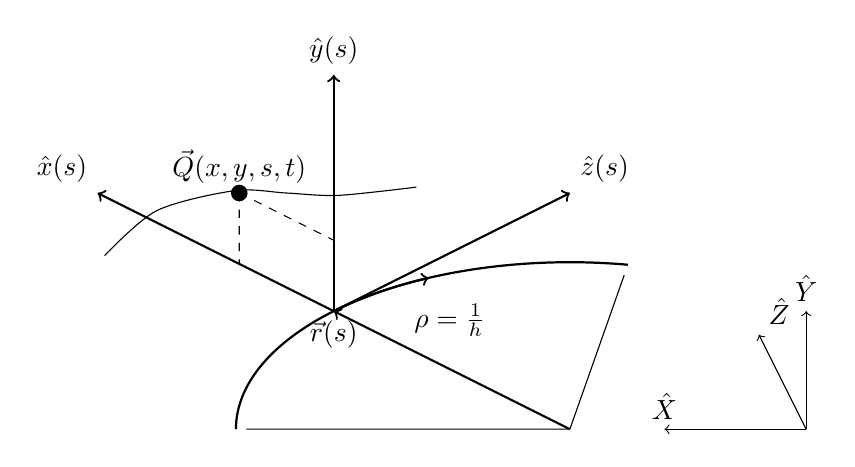
\begin{tikzpicture}[ scale=3, x={(-1cm,.5cm)}, y={(0cm,1cm)}, z={(1cm,.5cm)} ]

\path (0,0,0) coordinate (P0);
\path (-1.5,0,.5) coordinate (PR);
\draw (P0) node [below]{$\vec r(s)$};

%Axes
\draw[thick,->] (P0) -- +(1,0,0) node[above left]{$\hat x(s)$};
\draw[thick,->] (P0) -- +(0,1,0) node[above]{$\hat y(s)$};
\draw[thick,->] (P0) -- +(0,0,1) node[above right]{$\hat z(s)$};

%Design trajectory
\begin{scope}[canvas is xz plane at y=0]
     \path (-1,0) coordinate (P0);
     \draw [thick] (0,0) arc (0:-45:1cm) node (P1) {};
     \draw [thick,->] (0,0) arc (0:20:1cm) node[above] {};
     \draw [thick] (0,0) arc (0:55:1cm) node (P2) {};
     \draw (P1) -- (P0);
     \draw (P2) -- (P0);
     \draw [thick,->]  (P0) -- (0,0);
     \draw (-.3,.0) node [above right] {$\rho=\frac{1}{h}$};
\end{scope}
\draw [->] (PR) -- +(.3,0,-.3) node[above] {$\hat X$} ;
\draw [->] (PR) -- +(0,.5,0)   node[above] {$\hat Y$} ;
\draw [->] (PR) -- +(.5,0,.3)  node[above right] {$\hat Z$} ;

% Particle
\path (.4,.3,0) coordinate (P0);
\path (P0) node[above] {$\vec Q(x,y,s,t)$};

\fill (P0) circle (1pt);

\draw[dashed] (P0) -- (.4,0,0);
\draw[dashed] (P0) -- (0,.3,0);

\draw plot [smooth] coordinates {
     (.42,.3,-.55)
     (.50,.3,-.25)
     (.42,.3,-.0)
     (.4,.2,.2)
     (.38,.1,.4)
     (.25,.1,.6)
 };




\end{tikzpicture}
\caption{Moving reference frame $(\hat{x},\hat{y},\hat{z})$ parametrized by
$s(t)$. The trajectory of a particle $Q$ can be described by the coordinates
$(x,y,s,t)$.} \label{fig:frame}
\end{figure}

The speed, momentum, energy, rest mass, charge of a particle are indicated
by $v$, $P$, $E$, $m$ and $q$, respectively.  These quantities are
related by the following equations:
\begin{align}
  v&=\beta c &
  E^2-P^2c^2&=m^2c^4 &
  E & = \gamma mc^2 &
  Pc & =\beta E
\end{align}
where $\beta$ and $\gamma$ are the relativistic factors.

In a curvilinear reference frame defined by a constant curvature $h_x$ in the
$\hat X, \hat Z$ plane and parameterized by $s$  (see Fig. \ref{fig:frame}), the
position of the particle at a time $t$ can be written as:
\begin{align}
  \vec Q(t)= \vec r(s) + x \,\hat x(s) + y\, \hat y(s),
\end{align}
and therefore identified by the coordinates $s, x, y, t$ in the reference frame
defined by $\hat x(s)$ and $\hat y(s)$. In particle tracking, $s$ is normally
used as independent parameter and $t$ as a coordinate.

The electromagnetic fields {\bf E} and {\bf B} can be derived in a curvilinear
reference frame from the potentials $V(x,y,s,t)$ and $\mathbf{A}(x,y,s,t)$, where
\begin{align}
\mathbf{A}(x,y,s,t)=A_x(x,y,s,t) \hat x(s) + A_y(x,y,s,t) \hat y(s) + A_s(x,y,s,t) \hat z(s)
\end{align}
and for which:
\begin{align}
  \mathbf{E} & = -\nabla V - \frac{\partial \mathbf{A}}{\partial t} 
               = -\partial_x V \hat x - \partial_y V \hat y -
  \frac{1}{1+h x}  \partial_s V \hat z - \partial_t \mathbf{A}
\end{align}
\begin{align}
  \mathbf{B} = \nabla\times\mathbf{A} & =
  \left(\partial_y A_s - \frac{\partial_s  A_y}{1+h x} \right) \hat x +\cdots \\
  &\cdots+\left(\frac{\partial_s A_x}{1+h x}-\frac{h A_s}{1+h x}
  -\partial_x A_s \right)\hat y
  +\left(\partial_x A_y - \partial_y A_x \right) \hat z.
\end{align}
In this reference frame the canonical momenta are:
\begin{align}
  P_x&=m \gamma \dot x + q A_x, &
  P_y&=m \gamma \dot y + q A_y, &
  P_s&=m \gamma \dot s (1 + h x)^2 + q (1 + h x) A_s.
\end{align}
If $s(t)$ is monotonically increasing, it is possible to derive the equations
of motion using $s$ as the independent parameter and $t$ as a coordinate with
$-E$ as the conjugate momentum. Since in accelerators the orbits of the
particles are often a perturbation of the reference trajectory followed by a
particle with rest mass $m_0$, charge $q_0$, speed $\beta_0 c$ and momentum
$P_0$, one could use the following derived quantities that usually assume small
values:
\begin{align}
  \Delta s  &=s - \beta  ct &
  c\Delta t &=s/\beta_0 - ct &
  \sigma    &= s - \beta_0 ct \\
  \delta    &=\frac{P-P_0}{P_0} &
  p_t       &=\frac{E-E_0}{P_0 c} &
  p_\sigma  &=\frac{E-E_0}{\beta_0 P_0 c}.
\end{align}
and rescale the momenta according to:
\begin{align}
  p_x&=P_x/P_0 &
  p_y&=P_y/P_0 &
  p_s&=P_s/P_0  \\
  a_x &=qA_x/P_0&
  a_y &=qA_y/P_0&
  a_s &=qA_s/P_0.
\end{align}
The corresponding Hamiltonians, kept implicit for brevity, are:
\begin{align}
  H \left(x,p_x,y,p_y,\sigma,p_\sigma;s\right) &= p_\sigma - p_s\\
  H \left(x,p_x,y,p_y,c\Delta t,p_t;s\right) &= \frac{p_t}{\beta_0} - p_s\\
  H \left(x,p_x,y,p_y,\Delta s,\delta;s\right) &= \delta - p_s,
\end{align}
where
\begin{align}
  p_s&= (1+h x) \left(
    \sqrt{(1+\delta)^2 - (p_x-a_x )^2 - (p_y-a_y )^2} + a_s   \right) \\
  \frac{P}{P_0}&= 1+\delta =
  \sqrt{\left(\frac{E}{P_0c}\right)^2-\left(\frac{mc}{P_0}\right)^2}=
    \sqrt{p_t^2+\frac{2p_t}{\beta_0} +\frac{1}{\beta_0^2}
    \left(1-\frac{m^2}{m_0^2}\right)+1} \\
  \frac{E}{P_0c}&=
    \frac1{\beta_0}+p_t=
    %\frac1{\beta_0}+\beta_0 p_{\sigma}=
    \sqrt{\left(\frac{P}{P_0}\right)^2+\left(\frac{mc}{P_0}\right)^2}=
    \sqrt{\left(1+\delta\right)^2+ \left(\frac{m}{m_0}\right)^2
    \left(\frac1{\beta_0\gamma_0}\right)^2}
\end{align}
\begin{align}
  \left(1+\delta\right)^2 &=\beta_0^2p_{\sigma}^2+2p_{\sigma}+1 &
  \beta=\frac{Pc}E&=\frac{ 1+\delta}{1/{\beta_0}+p_t} \\
\end{align}

In addition the following derivatives and approximations can be derived:
\begin{align}
\delta &\simeq
      p_\sigma - \frac{1}{\gamma_0^2}\cdot\frac12 p_\sigma^2 &
\TnD{\delta}{p_\sigma}{}  &=
      \frac{\beta_0} \beta \simeq
      1- \frac{p_\sigma}{\gamma_0^2} &
\TnD{\delta}{p_\sigma}{2} &=
      -\frac{1}{\gamma_0^2} \cdot \left(\frac{p_0}{p}\right)^3 \\
\delta &\simeq
      \frac{p_t}{\beta_0} - \frac{1}{\beta_0^2\gamma_0^2}\cdot\frac12 p_t^2 &
\TnD{\delta}{p_t}{}  &=
      \frac{1}{\beta} \simeq
  \frac{1}{\beta_0}- \frac{p_t}{\beta_0^2\gamma_0^2} &
\TnD{\delta}{p_t}{2} &=
      -\frac{1}{\beta_0^2 \gamma_0^2} \cdot \left(\frac{p_0}{p}\right)^3 
\end{align}


\section{Beam-line elements tracking maps}
Each beam line elements is often characterized by a specific field
configuration which determine the way the equation of motions are solved. The
solutions of the equation of motion are typically explicit and derived by
solving exactly the Hamilton equations for arbitrary initial conditions of an
approximated Hamiltonian.

The following section illustrates the tracking maps used by SixTrack, labelled
by the beam line elements that the maps approximately represent. The map is the
solution of the equations of motion for a step $L$ in the independent parameter
$s$ with a given set of initial conditions in the canonical coordinates. For
brevity, when a coordinate is left unchanged by the map, the corresponding
equation is omitted.  High order integrators for single beam line elements can
be built by combining simpler maps (e.g. thin kick and drifts).

The following maps use the canonical conjugate pairs $(x,p_x)$, $(y,p_y)$ 
and $(\sigma,p_\sigma)$. It should be noted that SixTrack compute $x'$ and $y'$
during tracking instead of the momentum coordinates $p_x$ and $p_y$ and ($E$,
$E_0$), ($P$, $P_0$) instead of $p_\sigma$. The canonical variables are
used instead for the generation of linear and higher order symplectic maps
needed for action-angle variable transformations and Twiss parameter extraction.


\subsection{Drift}
A drift is a straight, field-free region ($h_{x,y}=0$, $V=0$ and
$\mathbf{A}=0$).  The exact and expanded Hamiltonian for a drift space are
\begin{align}
  H = p_\sigma - \sqrt{(1+\delta)^2 - p_x^2 - p_y^2} &\approx
  p_\sigma - \delta + \frac{1}{2}\frac{p_x^2+p_y^2}{1+\delta}.
\end{align}

With the help of the following definitions:
\begin{align}
   x_p&=\frac{P_x}{P_0 (1+\delta)}\simeq\frac{p_x}{p_z}=x', &
   y_p&=\frac{P_y}{P_0 (1+\delta)}\simeq\frac{p_y}{p_z}=y', %&
  %p_z&=\frac{P_z}{P_0}, &
  %\beta_z &= \beta \frac{P_z}{P}= \frac{\beta p_z}{1+\delta},
  %\beta_z &= \beta \frac{P_z}{P}= \frac{p_z}{\frac{1}{\beta_0}+p_t},
\end{align}


the map relative to the expanded Hamiltonian is (eq. 3.49 in \cite{ripken95})
\begin{align}
  x & \to x + x_p L &
  y & \to y + y_p L\\
  c\Delta t & \to c\Delta t + \frac{L}{\beta_0} - \frac{L}{\beta} 
  \left(1+\frac{x_p^2+y_p^2}{2}  \right) &
  \Delta s & \to \Delta s -\frac{x_p^2+y_p^2}{2} \\
  \sigma & \to \sigma +
  L - \beta_0 \frac{L}\beta
        \left( 1+\frac{x_p^2+y_p^2}{2}  \right)  .
\end{align}

\noindent With the additional definitions:
\begin{align}
   %'&=\frac{P_x}{P_z}=\frac{p_x}{p_z}, &
   %'&=\frac{P_y}{P_z}=\frac{p_y}{p_z}, &
  p_z&=\frac{P_z}{P_0}\\
  p_z&=\sqrt{(1+\delta)^2 - p_x^2 - p_y^2}=\sqrt{\beta_0^2p_{\sigma}^2+2p_{\sigma}+1 - p_x^2 - p_y^2}, \\
    %\beta_z &= \beta \frac{P_z}{P}= \frac{\beta p_z}{1+\delta},
  \beta_z &= \beta \frac{P_z}{P}=\frac{p_z}{1+\delta}= \frac{p_z}{1/\beta_0+p_t}=\frac{p_z}{1/\beta_0+\beta_0 p_\sigma},
\end{align}
the map of the exact Hamiltonian (eq. A.6a in \cite{heinemann95}) is
\begin{align}
  x      & \to x+x'L &
  y      & \to y+y'L \\
    c\Delta t     & \to c\Delta t + \left(\frac{1}{\beta_0}
  -\frac{1}{\beta_z}\right)\cdot L &
    \Delta s  & \to \Delta s+\frac{p_z-1-\delta}{p_z} \cdot L \\
  \sigma & \to \sigma + \left(1 - \frac{\beta_0}{\beta_z} \right) \cdot L &
  \sigma & \to \sigma + \frac{p_z -1 - \beta_0^2 p_\sigma}{p_z}  \cdot L.
\end{align}

It is possible to define a ``polar'' drift that has the effect of rotating the reference frame
\cite{forest99} for instance in the $x$-$z$ plane:
\begin{align}
p_x & \to   p_x \cos \theta + p_z \sin\theta &
p_z & \to - p_x \sin \theta + p_z \cos\theta \\
z   &= -x \sin \theta & x' &= p_x/p_z &  y' &= p_y/p_z \\
x   & \to x \cos\theta - x' z  &
y   & \to y - x' z  \\
\Delta s & \to \Delta s +\frac{1+\delta}{p_z} z &
\sigma & \to \sigma + \frac{\beta_0}{\beta_z}   z.
\end{align}
where $\theta$ is the angle bringing the new $\hat x$ towards the old $\hat z$.
The map can be also generated by combining a rotation with a $-x
\sin(\theta)$-length drift. This map is not used in SixTrack.


\subsection{Dipole}
In a curvilinear reference system with a constant curvature $h_x$ in the
horizontal plane or $h_y$ in the vertical plane (but not both, i.e. $h_x \cdot h_y=0$)
a uniform magnetic field can be derived by the vector potential:
\begin{align}
  A_x & = 0, & A_y & = 0, & A_s & = 
  - B_y x\left(1-\frac{h_xx}{2(1+h_xx)}\right),
\end{align}
where we have chosen $h_y=0$. Often the bending radius of the dipole correspond to 
$h_{x,y}=\frac{q_0}{p} B_{x,y}$, where $q_0$ is the charge of the reference particle, 
which simplify the Hamiltonian further. In these conditions the exact and
expanded Hamiltonian for a horizontal bending magnet is (eq. 2.12 in
\cite{barber87})
\begin{align}
  H &= p_\sigma - p_s + q\cdot h_xx \left(1+\frac{h_xx}{2}\right) \\
    &\approx p_\sigma + \frac{1}{2}\frac{p_x^2+p_y^2}{1+\delta}
  - h_xx(1+\delta) + \frac{q}{q_0} h_xx \left(1+\frac{h_xx}{2}\right)
\end{align}

\subsubsection{Thick dipole}
Defining the following quantities,
\begin{align}
  G_x&= \frac{q}{q_0} \cdot\frac{h_x^2}{1+\delta}, & G_y&= \frac{q}{q_0} \cdot\frac{h_y^2}{1+\delta} \\
  C_{x,y}&=\cos(\sqrt{G_{x,y}}L), & S_{x,y}&=\sin(\sqrt{G_{x,y}}L)
\end{align}
the map relative to the expanded Hamiltonian is (eq. 4.11 in \cite{barber87})
\begin{align*}
  x   &\to C_x \cdot x + \frac{S_x}{\sqrt{G_x}}\frac{1}{1+\delta} \cdot p_x + \frac{\delta}{h_x} (1 - C_x) \\
  p_x &\to -\sqrt{G_x} (1+\delta) \cdot S_x \cdot x + C_x \cdot p_x + \delta \sqrt{1+\delta} \cdot S_x \\
  y   &\to C_y \cdot y + \frac{S_y}{\sqrt{G_y}}\frac{1}{1+\delta} \cdot p_y + \frac{\delta}{h_y} (1 - C_y) \\
  p_y &\to -\sqrt{G_y} (1+\delta) \cdot S_y \cdot y + C_y \cdot p_y + \delta \sqrt{1+\delta} \cdot S_y \\
  \sigma &\to \sigma + L\left(1 - \frac{\beta_0}{\beta}\right) \\
  & \qquad\, -\frac{\beta_0}{\beta} \Bigg[ \frac{h_x S_x}{\sqrt{G_x}} \cdot x + \frac{1-C_x}{h_x} \cdot p_x
  + \frac{h_y S_y}{\sqrt{G_y}} \cdot y + \frac{1-C_y}{h_y} \cdot p_y
  + \delta \left(2L - \frac{S_x}{\sqrt{G_x}} - \frac{S_y}{\sqrt{G_y}} \right) \Bigg] \\
  & \qquad\, - \frac{1}{4}\frac{\beta_0}{\beta} \Bigg[ G_x \left(L-\frac{C_xS_x}{\sqrt{G_x}} \right)
  \left(x - \frac{\delta}{h_x}\right)^2
  + \left(L+\frac{C_xS_x}{\sqrt{G_x}} \right) \frac{p_x^2}{(1+\delta)^2}
  -\left(x-\frac{\delta}{h_x}\right) \frac{2S_x^2}{1+\delta} \cdot p_x \\
  & \qquad\, + G_y \left(L-\frac{C_yS_y}{\sqrt{G_y}} \right)
  \left(y - \frac{\delta}{h_y}\right)^2 + \left(L+\frac{C_yS_y}{\sqrt{G_y}}\right) 
  \frac{p_y^2}{(1+\delta)^2}
  -\left(y-\frac{\delta}{h_y}\right)\frac{2S_y^2}{1+\delta} \cdot p_y \Bigg].
\end{align*}
An alternative version of the ideal sector bend (eq. 12.18 in \cite{forest99}) with arbitrary bending field $b_1=\frac{q_0}{P_O} B_y$ and reference radius $\rho$ is
\begin{align}
  \alpha(s)&=\sin^{-1}\left(
  \frac{p_x(s)}{\sqrt{(1+\delta^2)-p_y^2}}\right)\\
  p_z(s) &= \sqrt{(1+\delta)^2-p_x^2(s) - p_y^2} \\
  x &\to \frac{\rho}{b_1}\left(\frac1\rho p_z(L)- p_x'(L) - b_1\right)\\
  p_x &\to p_x \cos(\theta) + \left(p_z(0)-b_1(\rho+x)\right)\sin(\theta)\\
  y &\to y+\frac{p_y L}{b_1 \rho}+
   \frac{p_y}{b_1}\left(\alpha(0)-\alpha(L)\right)\\
  ct &\to ct + \frac{(1+\delta)L}{b_1\rho}+
          \frac{(1+\delta)}{b_1}\left(\alpha(0)-\alpha(L) \right)
\end{align}
where $\theta=hL$ is the bending angle. This map is numerically unstable for $L\to0$, $b_1\to0$, $\rho\to\infty$.  This map is not used in SixTrack.


\subsubsection{Thin dipole}
The map for a thin dipole kick (horizontal or vertical) from the expanded Hamiltonian is 
(eq. 4.12 in \cite{heinemann95}):
\begin{align}
  p_x &\to p_x - \frac{q}{q_0} \cdot (h_xL)(1+h_xx) + (h_xL)(1+\delta) \\
  p_y &\to p_y - \frac{q}{q_0} \cdot (h_yL)(1+h_yy) + (h_yL)(1+\delta)\\
  \sigma &\to \sigma - \frac{\beta_0}{\beta} (h_xx + h_yy) L.
\end{align}

The map for a horizontal ($h_y=0$) thin dipole with the exact Hamiltonian
can be expressed as (eq. 3.21 in \cite{barber96})
$T_{II}(L/2)\circ T_I(L) \circ T_{II}(L/2)$ where $T_{II}(L)$ is given by
\begin{align}
    p_x &\to \frac{1}{1+(h_xL)^2} \left[p_x + (h_xL)(1+\delta) 
    \left(\sqrt{1-\frac{p_x^2+p_y^2-C}{(1+\delta)^2}}-1 \right)\right] \\
    x &\to x + (h_xL)\cdot x\cdot \frac{p_x}{p_z} \\
    y &\to y + (h_xL)\cdot x\cdot \frac{p_y}{p_z} \\
    \sigma &\to \sigma + (h_xL)\cdot x\cdot 
    \left(\frac{\beta_0}{\beta}-\frac{\beta_0}{\beta_z}\right),
\end{align}
with $C=-(h_xL)^2p_y^2+2(h_xL)(1+\delta)p_x$ and $T_{I}(L)$ is given by
\begin{align}
    p_x &\to p_x -h_x^2Lx + (h_xL)\cdot\delta \\
    \sigma &\to \sigma - (h_xL)x\cdot \frac{\beta_0}{\beta}.
\end{align}
In order to represent a dipole of length $L$ this map is to be combined with 
two surrounding drift spaces using the exact Hamiltonian, each of half the 
length of the dipole.

The exact thin dipole could be also generated by the composition of
\begin{align}
D(-L/2) \circ D_p(\theta/2) \circ K(L) \circ D_p(\theta/2) \circ  D(L/2)
\end{align}
for which $D$ is a drift, $D_p$ a polar drift and $K$ the map generated by
$ K=b_y(x +\frac{h_x}{2}x^2) $. This map is not used in SixTrack.

\subsubsection{Dipole Edge effects}
The dipole edge effects from a dipole of length $L$ and bending
angle $\theta$ can be approximated by the map:
\begin{align}
    p_x &\to p_x + \frac{1+\delta}{\rho} \tan(\alpha) \cdot x \\
    p_y &\to p_y - \frac{1+\delta}{\rho} \tan(\alpha) \cdot y,
\end{align}
where the bending radius $\rho$ and $\alpha$ are defined as
\begin{align}
    \rho^{-1}   &= \frac{h_x}{\sqrt{1+\delta}} &
    \alpha &= \frac{1}{2} \frac{L}{\rho} = \frac{\theta}{2}.
\end{align}.


\subsection{Quadrupole}

A quadrupole is characterized by the vector potential
\begin{align}
  a_x & = 0  & a_y & = 0 & a_s & = -\frac{1}{2}k_1(y^2 - x^2).
\end{align}
The expanded Hamiltonian for a particle in a quadrupole is
\begin{align}
  H =  p_\sigma -\delta + \frac{1}{2}\frac{p_x^2+p_y^2}{1+\delta}        %PH 15/02/11 added -\delta
  + \frac{1}{2}k_1(x^2 - y^2).
\end{align}

\subsubsection{Thick quadrupole}
\noindent By defining the following quantities
\begin{align}
  g &= q \cdot \frac{g_0}{1+\delta}
  %C &= \cos(\sqrt{g}L) & S &= \sin(\sqrt{g}L) \\
  %\hat{C} &= \cosh(\sqrt{g}L) & \hat{S} &= \sinh(\sqrt{g}L) ,
\end{align}
we have the following two cases
\begin{align}
    C &= \left\{
         \begin{array}{l l}
             \cos(\sqrt{g}L)  & g > 0 \\
             \cosh(\sqrt{-g}L) & g < 0
         \end{array}
         \right. &
    S &= \left\{
         \begin{array}{l l}
             \sin(\sqrt{g}L)  & g > 0 \\
             \sinh(\sqrt{-g}L) & g < 0
         \end{array}
         \right. \\
    \hat{C} &= \left\{
         \begin{array}{l l}
             \cosh(\sqrt{g}L)  & g > 0 \\
             \cos(\sqrt{-g}L) & g < 0
         \end{array}
         \right. &
    \hat{S} &= \left\{
         \begin{array}{l l}
             \sinh(\sqrt{g}L)  & g > 0 \\
             \sin(\sqrt{-g}L) & g < 0
         \end{array}
         \right.
\end{align}
Using the above definitions the map of a thick quadrupole is (eq. 4.2 in \cite{barber87})
\begin{align}
  x   &\to C \cdot x + \frac{S}{\sqrt{|g|}} \frac{p_x}{1+\delta} \\
  p_x &\to - (1+\delta) \sqrt{|g|} S \cdot x + C \cdot p_x \\
  y   &\to \hat C \cdot y + \frac{\hat S}{\sqrt{|g|}} \frac{p_y}{1+\delta} \\
  p_y &\to (1+\delta)\sqrt{|g|} \hat S \cdot y + \hat C \cdot p_y \\
  \sigma &\to \sigma + L \left(1 - \frac{\beta_0}{\beta} \right)
  - \frac{|g|}{4} \frac{\beta_0}{\beta} \Bigg[\left(L-\frac{C\cdot S}{\sqrt{|g|}} \right) \cdot x^2
  - \left(L-\frac{\hat{C}\cdot\hat{S}}{\sqrt{|g|}} \right) \cdot y^2 \Bigg] \\
  & \,\qquad- \frac{1}{4}\frac{\beta_0}{\beta} \Bigg[ \left(L
  + \frac{C\cdot S}{\sqrt{|g|}}\right) \cdot \frac{p_x^2}{(1+\delta)^2}
  + \left(L + \frac{\hat{C}\cdot\hat{S}}{\sqrt{|g|}} \right) \frac{p_y^2}{(1+\delta)^2} \Bigg] \\
  & \,\qquad- \frac{1}{2}\frac{\beta_0}{\beta}\Bigg[-x\cdot\frac{p_x}{1+\delta} \cdot S^2 
  + y\cdot\frac{p_y}{1+\delta} \hat{S}^2 \Bigg].
\end{align}

\subsubsection{Thick skew quadrupole}
The Hamiltonian for a skew quadrupole
\begin{align}
    H = p_\sigma-\delta+\frac{1}{2}\frac{p_x^2+p_y^2}{1+\delta}-N\cdot xy,
\end{align}
where $N=\frac{1}{2}\frac{q}{E_0}\left(\frac{\partial B_x}{\partial x} - 
\frac{\partial B_y}{\partial y}\right)_{x=y=0}$.
For a thick skew quadrupole the map is (eq. 3.19, 3.20 in \cite{ripken85})
\begin{align}
    x &\to C^+\cdot x+S^+\cdot p_x-C^-\cdot y-S^-\cdot p_y \\
    p_x &\to -\hat{S}^-\cdot x+C^+\cdot p_x+\hat{S}^+\cdot y-C^-\cdot p_y \\
    y &\to -C^-\cdot x-S^-\cdot p_x+C^+\cdot y+S^+\cdot p_y \\
    p_y &\to \hat{S}^+\cdot x -C^-\cdot p_x -\hat{S}^-\cdot y + C^+\cdot p_y \\
    \sigma &\to \sigma + \frac{1}{8}(x^2+y^2)\left(C^+\hat{S}^-+C^-\hat{S}^+\right) \\
    &\qquad-\frac{1}{8}\frac{p_x^2+p_y^2}{(1+\delta)^2}\left[L+C^+S^++C^-S^-\right] \\
    &\qquad+\frac{1}{2}Nxy\left[L-C^+S^+-C^-S^-\right] 
    +\frac{1}{2} \frac{p_xp_y}{(1+\delta)^2} \left[C^+S^-+C^-C^+\right] \\
    &\qquad+\frac{xp_x+yp_y}{1+\delta}S^+\hat{S}^--\frac{xp_y+p_xy}{1+\delta}\frac{1}{2}
    \left[S^+\hat{S}^-+S^-\hat{S}^+\right]
\end{align}
where 
\begin{align}
    C^-&=\frac{\cos\sqrt{N}L-\cosh\sqrt{N}L}{2} &
    C^+&=\frac{\cos\sqrt{N}L+\cosh\sqrt{N}L}{2} \\
    S^-&=\frac{\sin\sqrt{N}L-\sinh\sqrt{N}L}{2\sqrt{N}} &
    S^+&=\frac{\sin\sqrt{N}L+\sinh\sqrt{N}L}{2\sqrt{N}} \\
    \hat{S}^-&=\frac{\sqrt{N}}{2}(\sin\sqrt{N}L-\sinh\sqrt{N}L) &
    \hat{S}^+&=\frac{\sqrt{N}}{2}(\sin\sqrt{N}L+\sinh\sqrt{N}L)
\end{align}

\subsection{Combined function magnet}

\subsubsection{Thin combined function magnet}
The map is the combination of the map for the thin dipole and for a thin quadrupole using 
the thin multipole expansion (eq. 3.12 in \cite{ripken95})
\begin{align}
  p_x &\to p_x - G_1 L \cdot x + (1+\delta)h_x L - q\cdot h_xL \\
  p_y &\to p_y - G_2 L \cdot y +(1+\delta) h_y L - q\cdot h_yL\\
  \sigma &\to \sigma - \frac{\beta_0}{\beta}(h_xx+h_yy) L,
\end{align}
where $G_1=q \cdot h_x^2+k_1$ and $G_2=q \cdot h_y^2-k_1$.


\subsection{Thin Multipole}
A longitudinally uniform static magnetic field can be described by the following equations
\begin{align}
  A_z&= - \Re \sum_{n=1} \frac1n \left(B_n+iA_n\right) 
    \frac{(x+iy)^n}{r_0^{n-1}}\\
    B_y+iB_x&=\sum_{n=1} \left(B_n+iA_n\right) \frac{(x+iy)^{n-1}}{r_0^{n-1}}.
\end{align}
A thin multiple idealize the effect of the field by taking the limit of the integration 
length going to zero while keeping constant the integrated strength. The Hamiltonian is:
\begin{align}
  H=- \delta(s) L \frac qp A_z.
\end{align}
The corresponding map is:
\begin{align}
  p_x &\to p_x - L\cdot\Re\left[\sum_{n=0} \frac{1}{n!} (k_n + i\hat k_n) (x+iy)^n \right], \\
  p_y &\to p_y + L\cdot\Im\left[\sum_{n=0} \frac{1}{n!} (k_n + i\hat k_n) (x+iy)^n \right],
\end{align}
for which
\begin{align}
  k_n&= \frac qp \PnD{B_y}{x}{n}
         = \frac qp \frac{n!}{r_0^n}  B_{n+1} &
  B_{n+1}= \frac {r_0^n}{n!}   \PnD{B_y}{x}{n} \\
  \hat k_n&= \frac qp \PnD{B_x}{x}{n}
         = \frac qp \frac{n!}{r_0^n}  A_{n+1} &
  A_{n+1}= \frac {r_0^n}{n!}   \PnD{B_x}{x}{n}
\end{align}
For instance, the map for a normal quadrupole, sextupole and octupole are :
\begin{align}
  p_x & \to p_x - L \cdot {k_1}\cdot x &
  p_y & \to p_y + L \cdot {k_1}\cdot y, \\
  p_x & \to p_x - L \cdot \frac{k_2}{2}\cdot (x^2-y^2) &
  p_y & \to p_y + L \cdot k_2 \cdot xy,\\
  p_x & \to p_x - L \cdot \frac{k_3}{6}\cdot(x^3 - 3xy^2) &
  p_y & \to p_y + L \cdot \frac{k_3}{6}\cdot(3x^2y - y^3) .
\end{align}

\subsection{RF-cavity}
The expanded Hamiltonian for a RF-cavity is (eq. 2.30 in \cite{ripken95})
\begin{align}
  H & = p_\sigma
  + \frac{1}{\beta_0^2} \frac{C}{2\pi h_a} \frac{qV(s)}{E_0} 
  \cos\left(h_a\frac{2\pi}{C}\sigma+\varphi\right),
\end{align}
where $h_a$ is the harmonic number, $\varphi$ is the phase angle, $V$ is the voltage and 
$C$ is the design circumference length. The thin lens transfer map is (eq. 3.44 in \cite{ripken95})
\begin{align}
  p_\sigma &\to p_\sigma + \frac{1}{\beta_0^2}\frac{qV(s_0)}{E_0} \cdot 
  \sin\left(h_a\frac{2\pi}{C}\sigma+\varphi\right).
\end{align}
Using the relation between $p_\sigma$ and the energy $E$, the map can be expressed as
the change in energy of the tracked particle
\begin{align}
  E &\to E + q\cdot V \sin\left(h_a\frac{2\pi}{C}\sigma+\varphi\right).
\end{align}
This is how Sixtrack performs the calculation.

\subsection{Solenoid}
The expanded Hamiltonian for a particle in a solenoid is
\begin{align}
  H &= p_\sigma+\frac{1}{2}\frac{(p_x+R\cdot y)^2+(p_y-R\cdot x)}{1+\delta},
\end{align}
where $R=\frac{1}{2}\frac{q}{P_0c}\mathbf{B}(0,0,s)$. The map for a solenoid 
of length $L$ in the thin lens approximation with the expanded 
Hamiltonian (eq. 4.35 in \cite{heinemann95})
\begin{align}
  x   &\to \,\,\,\,\, C\cdot x + S\cdot y \\
  p_x &\to -\theta R\cdot C \cdot x+C\cdot p_x
        -\theta R\cdot S\cdot y+S\cdot p_y \\
  y   &\to -S\cdot x + C\cdot y \\
  p_y &\to \,\,\,\,\, \theta R\cdot S\cdot x - S\cdot p_x 
  - \theta R\cdot C \cdot y + C\cdot p_y \\
  \sigma &\to \sigma - \frac{\beta_0}{\beta}
  \frac{\theta}{1+\delta} \left(\frac{1}{2}
  R (x^2 + y^2) + (p_xy - p_yx)\right)
\end{align}
where $R\equiv R(s_0)$, $\theta=\frac{R}{1+\delta}$, 
$C=\cos(\theta)$ and $S=\sin(\theta)$.\\[0.5em]
The map for a thick solenoid is (eq. 3.47, 3.48 in \cite{ripken85}) 
\begin{align}
    x &\to C^2 \cdot x+\frac{1}{R}\cdot S\cdot C\cdot p_x+S\cdot C\cdot y
    + \frac{1}{R}\cdot S^2 \cdot p_y \\
    p_x &\to -R\cdot S\cdot C\cdot x + C^2\cdot p_x
    -R\cdot S^2\cdot y + S\cdot C\cdot p_y \\
    y &\to -S\cdot C\cdot x -\frac{1}{R}\cdot S^2 \cdot p_x
    +C^2\cdot y + \frac{1}{R}\cdot S\cdot C\cdot p_y \\
    p_y &\to R\cdot S^2\cdot x -S\cdot C\cdot p_x
    -R\cdot S\cdot C\cdot y + C^2\cdot p_y \\
    \sigma &\to \sigma - \frac{L}{2} \left[R^2(x^2+y^2)+2R\left(
    \frac{p_x}{1+\delta}y - \frac{p_y}{1+\delta}x\right) 
    + \frac{p_x^2+p_y^2}{(1+\delta)^2} \right]
\end{align}
where $\theta=R\cdot L$, $C=\cos\theta$ and $S=\sin\theta$.

\subsection{Beam-beam lens}
In order to study beam-beam interactions the strong bunch can be split
longitudinally into several slices, each slice described by an electrostatic
potential of the form (eq. 2.1 in \cite{beam_beam})
\begin{align}
    \hat{U}(x,y;\hat{\Sigma}_{11},\hat{\Sigma}_{33};\theta) \equiv
    U(\hat{x},\hat{y};\hat{\Sigma}_{11},\hat{\Sigma}_{33}) =
    -\frac{r_p}{\gamma_0} \int_0^\infty 
    \frac{\exp\left(-\frac{\hat{x}^2}{2\hat{\Sigma}_{11}+u}
    -\frac{\hat{y}^2}{2\hat{\Sigma}_{33}+u}\right)}{\sqrt{2\hat{\Sigma}_{11}+u}
    \sqrt{2\hat{\Sigma}_{33}+u}} du,
\end{align}
where $\Sigma_{ij}$ are the elements of the $6\times 6$ phase-space envelope
matrix of the strong bunch.

To evaluate the effect of the beam-beam interaction on a test particle two
sets of transformations need to be considered. The first is a transformation
of Cartesian to accelerator coordinates and a Lorentz boost making the
collision between the bunches head-on, this is accomplished by the Lorentz
transformation given by (eq. 2.21 in \cite{beam_beam})
\begin{equation}
    \mathcal{L} = \left(
        \begin{array}{cccc}
            \frac{1}{\cos\phi} & -\cos\alpha\sin\phi & 
            -\tan\phi\sin\phi & -\sin\alpha\sin\phi \\
            -\cos\alpha\tan\phi & 1 & \cos\alpha\tan\phi & 0 \\
            0 & -\cos\alpha\sin\phi & \cos\phi & -\sin\alpha\sin\phi \\
            -\sin\alpha\tan\phi & 0 & \sin\alpha\tan\phi & 1
        \end{array}
    \right),
\end{equation}
where $\alpha$ is the crossing plane angle and $2\phi$ is the total crossing
angle.  The second set of transformations is called the Synchro-Beam Mapping
(SBM). In the SBM the test particle at the interaction point (IP) is brought
to the collision point by a drift, then the beam-beam interaction is applied
and finally the position of the test particle is brought back to the IP.

For a test particle with Lorentz transformed coordinates
$(x^*,p_x^*,y^*,p_y^*,z^*,p_z^*)$ the explicit form for the SBM is (eq. 2.65
in \cite{beam_beam})
\begin{align}
    x^* &\to x^* + Sn^*F_x^* \\
    p_x^* &\to p_x^*-n^*F_x^* \\
    y^* &\to y^* + Sn^*F_y^* \\
    p_y^* &\to p_y^* - n^*F_y^* \\
    p_z^* &\to p_z^* -n^*F_z^*- \frac{1}{2} 
    \left[n^*F_x^*(p_x^*-\frac{1}{2}n^*F_x^*)
    +n^*F_y^*(p_y^*-\frac{1}{2}n^*F_y^*)\right],
\end{align}
where $n^*$ is the number of particles in the slice $S$ is the distance between
a test particle and the strong bunch and
\begin{align}
    F_x^* &= \frac{\partial}{\partial\bar{x}^*} 
    \hat{U}(\bar{x}^*,\bar{y}^*;\hat{\Sigma}_{11}(\varphi),
    \hat{\Sigma}_{33}(\varphi);\theta(\varphi)) \\
    F_y^* &= \frac{\partial}{\partial\bar{y}^*} 
    \hat{U}(\bar{x}^*,\bar{y}^*;\hat{\Sigma}_{11}(\varphi),
    \hat{\Sigma}_{33}(\varphi);\theta(\varphi)) \\
    F_z^* &= \frac{\partial}{\partial\bar{z}^*} 
    \hat{U}(\bar{x}^*,\bar{y}^*;\hat{\Sigma}_{11}(\varphi),
    \hat{\Sigma}_{33}(\varphi);\theta(\varphi)),
\end{align}
which are calculated from the expression for $\hat{U}$ given above. Finally the
inverse Lorentz transformation $\mathcal{L}^{-1}$ is applied to the SBM transformed 
coordinates.

\subsection{Beam-beam element}
In the following, $r_e$ is the classical electron radius and $S$ is the strength ratio with respect to the nominal beam-beam kick strength. The maps below assumes no linear coupling between the transverse planes.

\subsubsection{Round beam}
Definitions
\begin{align}
	r_x &= x - x_{\text{co}} + x_{\text{sep}}, \\
    r_y &= y - y_{\text{co}} + y_{\text{sep}}, \\
    r^2 &= r_x^2+r_y^2.
\end{align}
The kick is
\begin{align}
	p_x &\to p_x + r_e\cdot S\cdot\frac{r_x}{r^2}\left[1-\exp\left(\frac{r^2}{2\sigma^2}\right)\right]-\text{beamoff(4)}, \\
    p_y &\to p_y + r_e\cdot S\cdot\frac{r_y}{r^2}\left[1-\exp\left(\frac{r^2}{2\sigma^2}\right)\right]-\text{beamoff(5)}.
\end{align}

\subsubsection{Elliptical beam}
For this map, it is assumed that $x>y$ (i.e. the horizontal extension of the beam is larger than the vertical extension.) For the reverse case, $y>x$, interchange $x$ and $y$ in the map.
\begin{align}
	r_x &= x - x_{\text{co}} + x_{\text{sep}}, \\
    r_y &= y - y_{\text{co}} + y_{\text{sep}}, \\
    \bar{\sigma} &= \sqrt{2(\sigma_x^2-\sigma_y^2)}.
\end{align}
The kick is
\begin{align}
	p_x &\to p_x + \sgn(r_x)\left[r_e\cdot S \frac{\sqrt{\pi}}{\bar{\sigma}}\left(\erf\left(\frac{|r_y|}{\bar{\sigma}}\right) - \exp\left(-\frac{1}{2}\left[\frac{r_x^2}{\sigma_x^2}+\frac{r_y^2}{\sigma_y^2}\right]\right) \erf\left(\frac{\sigma_x}{\sigma_y}\frac{|r_y|}{\bar{\sigma}}\right) \right) \right] -\text{beamoff(4)}, \\
    p_y &\to p_y + \sgn(r_y)\left[r_e\cdot S \frac{\sqrt{\pi}}{\bar{\sigma}}\left(\erf\left(\frac{|r_x|}{\bar{\sigma}}\right) - \exp\left(-\frac{1}{2}\left[\frac{r_x^2}{\sigma_x^2}+\frac{r_y^2}{\sigma_y^2}\right]\right) \erf\left(\frac{\sigma_y}{\sigma_x}\frac{|r_x|}{\bar{\sigma}}\right) \right) \right] -\text{beamoff(5)}.
\end{align}



\subsection{Hirata's beam-beam element}
Initial transformation of coordinates.
\begin{align}
    x_i      & \to (x + dx) - x_{\text{co}} \\
    p_{x,i}  & \to p_x - p_{x,\text{co}} \\
    y_i      & \to (y + dy) - y_{\text{co}} \\
    p_{y,i}  & \to p_y - p_{y,\text{co}} \\
    \sigma_i &\to \sigma-\sigma_{\text{co}} \\
    \delta_i &\to \delta-\delta_{\text{co}}.
\end{align}

Lorentz boost. $\phi$ is the crossing plane angle and $\alpha$ is the half crossing angle. The particle has initial coordinates $(x^i,p_x^i,y^i,p_y^i,\sigma^i,\delta^i)$.
We define $h=(1+\delta^i)-\sqrt{(1+\delta^i)^2-(p_x^i)^2-(p_y^i)^2}$. $p_z$ is computed with the most recent values of $\delta$, $p_x$ and $p_y$.
\begin{align}
    \delta &\to \delta^i - \cos\alpha\tan\phi\cdot p_x^i - \sin\alpha\tan\phi\cdot p_y^i + h\cdot\tan^2\phi \\
    p_x &\to p_x^i \frac{1}{\cos\phi}\left(p_x^i-\tan\phi\cos\alpha\cdot h\right) \\
    p_y &\to p_y^i \frac{1}{\cos\phi}\left(p_y^i-\tan\phi\sin\alpha\cdot h\right) \\
    \sigma &\to \frac{\sigma^i}{\cos\phi} + \left(1-\frac{1+\delta}{p_z}\right)\left(\sin\phi\cos\alpha\cdot x^i+\sin\phi\sin\alpha\cdot y^i\right) \\
    x &\to \cos\alpha\tan\phi\cdot\sigma + \left(1+\cos\alpha\sin\phi\frac{p_x}{p_z}\right)\cdot x^i +\sin\alpha\sin\phi\frac{p_x}{p_z}\cdot y^i \\
    y &\to \sin\alpha\tan\phi\cdot\sigma + \left(1+\sin\alpha\sin\phi\frac{p_y}{p_z}\right)\cdot y^i +\cos\alpha\sin\phi\frac{p_y}{p_z}\cdot x^i
\end{align}

Inverse Lorentz boost. We define the determinat of the inverse Lorentz transformation matrix as
\begin{align}
    D &= \frac{1}{\cos\phi} + \tan\phi \left[\frac{p_x^i}{p_z}\cos\alpha+\frac{p_y^i}{p_z}\sin\alpha-\left(1-\frac{1+\delta^i}{p_z}\right)\sin\phi\right].
\end{align}

\begin{align}
    x &\to \frac{1}{D}\bigg[ x\left(\frac{1}{\cos\phi}+\sin\alpha\tan\phi\left(\frac{p_y}{p_z}-\sin\alpha\sin\phi\left(1-\frac{1+\delta}{p_z}\right)\right)\right) \\
    &\qquad\qquad + y\sin\alpha\tan\phi\left(\left(1-\frac{1+\delta}{p_z}\right)\cos\alpha\sin\phi-\frac{p_x}{p_z}\right) \\
    &\qquad\qquad - \sigma\tan\phi\left(\cos\alpha+\sin\phi\cos\alpha\sin\alpha\frac{p_y}{p_z}-\sin^2\alpha\sin\phi\frac{p_x}{p_z}\right)\bigg] \\
    y &\to \frac{1}{D}\bigg[ y\left(\frac{1}{\cos\phi}+\cos\alpha\tan\phi\left(\frac{p_x}{p_z}-\cos\alpha\sin\phi\left(1-\frac{1+\delta}{p_z}\right)\right)\right) \\
    &\qquad\qquad + y\cos\alpha\tan\phi\left(\left(1-\frac{1+\delta}{p_z}\right)\sin\alpha\sin\phi-\frac{p_y}{p_z}\right) \\
    &\qquad\qquad - \sigma\tan\phi \left(\sin\alpha+\sin\phi\cos\alpha\sin\alpha\frac{p_x}{p_z}-\cos^2\alpha\sin\phi\frac{p_y}{p_z}\right)\bigg] \\
    \sigma &\to \frac{1}{D}\bigg[\sigma\left(1+\frac{p_x}{p_z}\cos\alpha\sin\phi+\frac{p_y}{p_z}\sin\alpha\sin\phi\right)
    -x\left(1+\frac{1+\delta}{p_z}\right)\cos\alpha\sin\phi \\
    &\qquad\qquad -y\left(1-\frac{1+\delta}{p_z}\right)\sin\alpha\sin\phi\bigg] \\
    \delta &\to \delta + \cos\alpha\sin\phi\cdot p_x + \sin\alpha\sin\phi\cdot p_y \\
    p_x &\to p_x + \cos\alpha\sin\phi\cos^3\phi\left[(1+\delta)-p_z^i\right] \\
    p_y &\to p_y + \sin\alpha\sin\phi\cos^3\phi\left[(1+\delta)-p_z^i\right]
\end{align}

\subsection{RF multipole}
The Hamiltonian for a thin RF multipole is
\begin{align}
    H &= \delta\left(s-\frac{L}{2}\right) \bigg\{-\frac{1}{k_{\rm RF}}
    \frac{qV_{\rm RF}}{p_s c}\cos(\vartheta_{\rm RF}-k_{\rm RF}z) + \cdots \\
    &\cdots+ \sum_{n=0}^N \frac{1}{(n+1)!}\Re\left[(K_{\text{N},n}L
    \cos(\vartheta_n-k_{\rm RF}z)+iK_{\text{S},n}L\cos(\varphi_n-k_{\rm RF}z))
    (x+iy)^{n+1}\right]\bigg\}
\end{align}
where the $n$-th order normal- and skew- multipole magnetic strengths are
\begin{align}
    K_{\rm N,n} &= \frac{q}{p_s} \frac{\partial^n B_y}{\partial x^n},
    & K_{\rm S,n} &= \frac{q}{p_s} \frac{\partial^n B_x}{\partial x^n},
\end{align}
respectively. The multipolar expansion is done similar as for a static
magnetic field, but to account for the oscillatory behaviour the multipolar
coefficients are expressed as
\begin{align}
    \tilde{B}_n(z)&=\Re[B_ne^{j(\vartheta_n-k_{\rm RF}z)}]=B_n\cos(\vartheta_n-k_{\rm RF}z)\\
    \tilde{A}_n(z)&=\Re[A_ne^{j(\varphi_n-k_{\rm RF}z)}]=A_n\cos(\varphi_n-k_{\rm RF}z),
\end{align}
where $\vartheta_n$ and $\varphi_n$ are the phases for the normal and skew
coefficients, $\tilde{B}_n(z)$ and $\tilde{A}_n(z)$, respectively, $k_{\rm
RF}$ is the RF wave number of the generating field ($k_{\rm RF}z=\omega_{\rm
RF}t$).

The kick experienced by an arbitrary particle in $(x,y,z)$ can be expressed as
(eq. 16 in \cite{rf_multipoles})
\begin{align}
    \Delta p_x &= -\sum_{n=0}^N \frac{1}{n!} \Re\left[(K_{\text{N},n}L\cos(\vartheta_n
    -k_{\rm RF}z) + iK_{\text{S},n}L\cos(\varphi_n-k_{\rm RF}z))(x+iy)^n\right], \\
    \Delta p_y &= \sum_{n=0}^N \frac{1}{n!} \Im\left[(K_{\text{N},n}L\cos(\vartheta_n
    -k_{\rm RF}z) + iK_{\text{S},n}L\cos(\varphi_n-k_{\rm RF}z))(x+iy)^n\right], \\
    \Delta p_t &= \frac{qV_{\rm RF}}{p_sc}\sin(\vartheta_{\rm RF}-k_{\rm RF}z)+\cdots \\
    & \qquad\cdots - k_{\rm RF}\sum_{n=0}^N \Re\left[(K_{\text{N},n}L\sin(\vartheta_n
    -k_{\rm RF}z) + iK_{\text{S},n}L\sin(\varphi_n-k_{\rm RF}z))(x+iy)^n\right].
\end{align}

In Sixtrack the following equations are used:

\begin{align}\Delta x' & =\frac{b_{2}\, x\,\cos\left(\phi+k\, z\right)}{1+\delta}\\
\Delta y' & =\frac{-b_{2}\, y\,\cos\left(\phi+k\, z\right)} {1+\delta} \\
\Delta E & =-P_0 k\beta_0\,\frac{b_{2}}{2}\,\left(x^{2}-y^{2}\right)\,\sin\left(\phi+k\, z\right)
\end{align}

 \begin{align}\Delta x' & =\frac{b_{3}\,\left(x^{2}-y^{2}\right)\,\cos\left(\phi+k\, z\right)}{1 + \delta}\\
\Delta y' & =\frac{-2b_{3}\, xy\,\cos\left(\phi+k\, z\right)}{1 + \delta}\\
\Delta E & =-P_0 k\beta_0\,\frac{b_{3}}{3}\,\left(x^{3}-3xy^{2}\right)\,\sin\left(\phi+k\, z\right)
\end{align}

 \begin{align}\Delta x' & =\frac{b_{4}\,\left(x^{3}-3xy^{2}\right)\,\cos\left(\phi+k\, z\right)}{1 + \delta}\\
\Delta y' & =\frac{-b_{4}\,\left(3x^{2}y-y^{3}\right)\,\cos\left(\phi+k\, z\right)}{1 + \delta}\\
\Delta E & =-\frac{P_0 k}{c}\,\frac{b_{4}}{4}\,\left(x^{4}-6x^{2}y^{2}+y^{4}\right)\,\sin\left(\phi+k\, z\right)
\end{align}

 \begin{align}\Delta x' & =\frac{a_{2}\, y\,\cos\left(\phi+k\, z\right)}{1 + \delta}\\
\Delta y' & =\frac{a_{2}\, x\,\cos\left(\phi+k\, z\right)}{1 + \delta}\\
\Delta E & =P_0 k\beta_0\, a_{2}\, xy\,\sin\left(\phi+k\, z\right)
\end{align}

 \begin{align}\Delta x' & =\frac{2a_{3}\, xy\,\cos\left(\phi+k\, z\right)}{1 + \delta}\\
\Delta y' & =\frac{-a_{3}\,\left(y^{2}-x^{2}\right)\,\cos\left(\phi+k\, z\right)}{1 + \delta}\\
\Delta E & =\frac{P_0 k\beta_0a_{3}}{3}\,\left(y^{3}-3yx^{2}\right)\,\sin\left(\phi+k\, z\right)
\end{align}

 \begin{align}\Delta x' & =\frac{a_{4}\,\left(y^{3}-3yx^{2}\right)\,\cos\left(\phi+k\, z\right)}{1 + \delta}\\
\Delta y' & =\frac{a_{4}\,\left(3xy^{2}-x^{3}\right)\,\cos\left(\phi+k\, z\right)}{1 + \delta}\\
\Delta E & =-P_0 k\beta_0\, a_{4}\,\left(x^{3}y-y^{3}x\right)\,\sin\left(\phi+k\, z\right),
\end{align}
, where $k = \frac{2\pi f}{c\beta_0} $, $f$ is frequency and $c$ is the speed of light. 

\subsection{Wire}
\label{sec:wire}
The wire element is described by in total 7 parameters: the wire current $I$, the physical length of the wire $L$ and the length of the embedded drift $L_{\mathrm{emb}}$, the horizontal distance $dx$ and vertical distance $dy$ between the wire midpoint and the closed orbit, and the tilt angle $\phi$ in the $(z,y)$ plane and the tilt angle $\theta$ in the $(x,z)$ plane. The length $L$ is the physical length of the wire while the embedded drift is the length of the integration interval of the kick (Eqn.~\ref{wire:eqn:5}) in order to also take the fringe fields of the wire into account. This is illustrated in Fig.~\ref{wire:fig:1} which shows the vector potential and magnetic field together with the physical length $L$ and the length of the embedded drift $L_{\mathrm{emb}}$. The tilt angles are illustrated in Fig.~\ref{wire:fig:2}.
\begin{figure}[t]
	\begin{minipage}{0.5\linewidth}
			\centering
			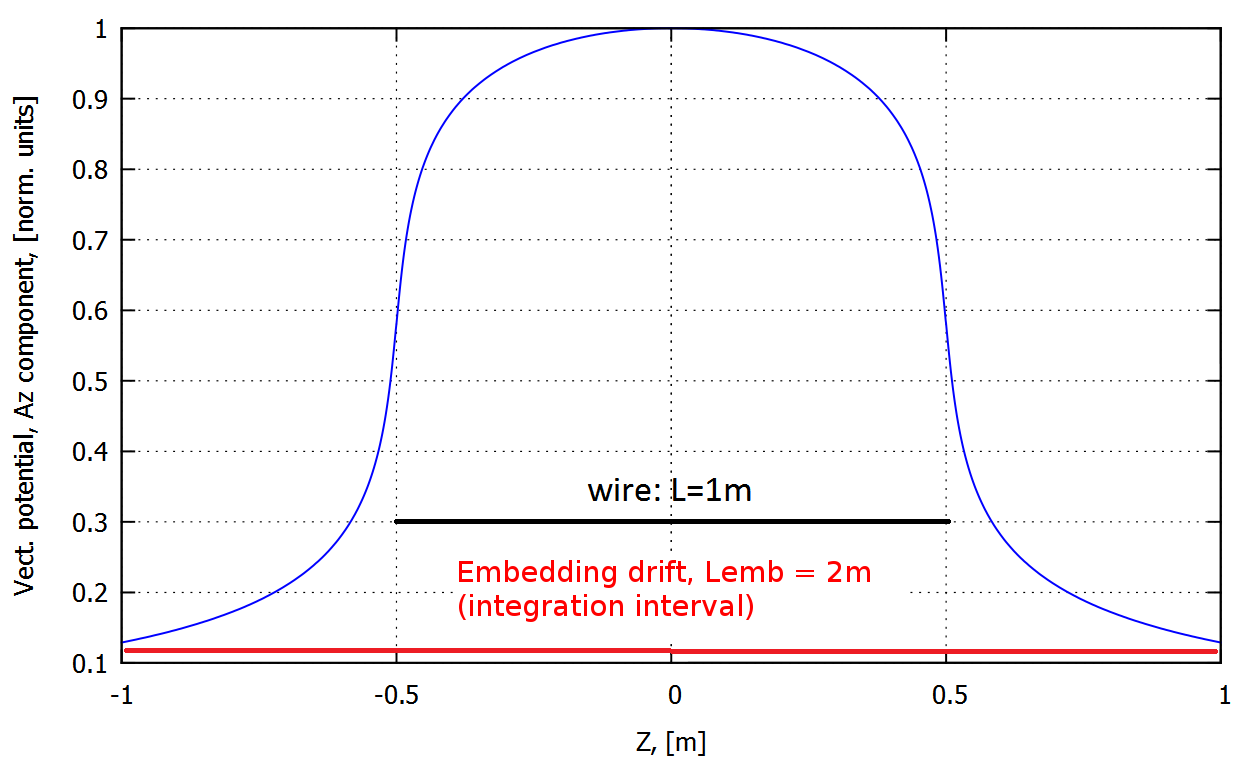
\includegraphics[width=1\linewidth]{wire_vector_potential.png}
	\end{minipage}
	\begin{minipage}{0.5\linewidth}
		\centering
		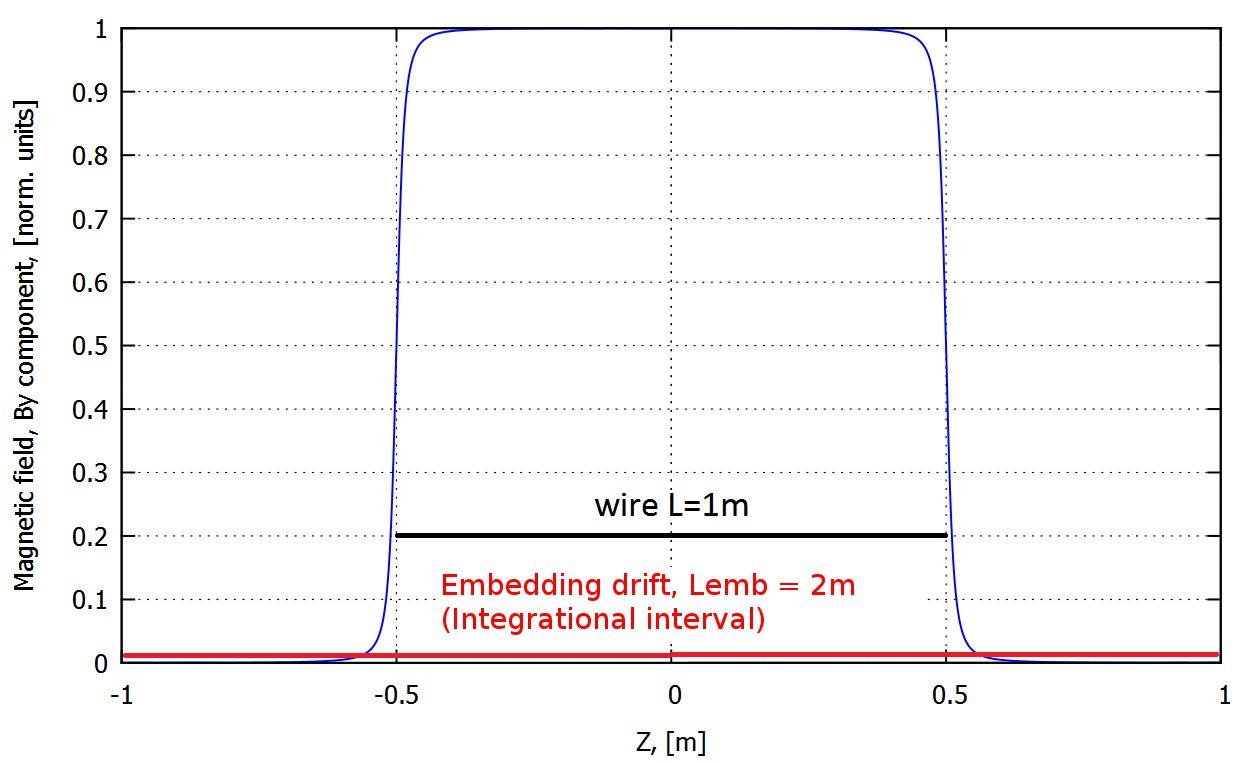
\includegraphics[width=1\linewidth]{wire_field.png}
	\end{minipage}
	\caption{Vector potential (left) and magnetic field (right) of a current bearing wire with physical length $L=1$~m and embedded drift (integrational length) $L_{\mathrm{emb}}=2$~m.\label{wire:fig:1}}
\end{figure}

To calculate the kick strength $\mathcal{L}$ of the wire in order to compensate the beam-beam kick from one long-range beam-beam encounter, the following relation between holds \cite{Valishev:wire}:
\begin{equation}
	\mathcal{L}=e\cdot c\cdot N_p=L\cdot I
\end{equation}
with $N_p$ being the bunch charge and $L$ and $I$ are the length and current of the wire. $\mathcal{L}$ than has to units Am.

The generic formula for a vector potential of a straight current bearing wire with length $L$ and current $I$ centered at the origin is given in Cartesian coordinates by the following expression\footnote{Note that Curvilinear and Cartesian coordinate system are equivalent as the curvature is zero at the location of the wire element.}: 
\begin{align}\label{wire:eqn:1}
	{A_i(x,y,z)} &=\frac{I\mu_0\cos(c_i)}{4\pi}\cdot\nonumber\\
	&\quad \left(\asinh\left(\frac{L/2-a}{\sqrt{b-a^2}}\right)-\asinh\left(\frac{-L/2-a}{\sqrt{b-a^2}}\right)\right), \ i=x,y,z, 
\end{align}
where the parameters $a$ and $b$ are defined as
\begin{align}\label{wire:eqn:2}
a&=x\cdot\cos(c_x)+y\cdot\cos(c_y)+z\cdot\cos(c_z), \\
b&=x^2+y^2+z^2,
\end{align}
and $\cos(c_i)$ are the direction cosines. The direction cosines can in general be expressed through two tilt angles $\phi$ and $\theta$ (see Fig.~\ref{wire:fig:2}) with:
\begin{align}\label{wire:eqn:3}
\cos(c_x)  &:= \frac{\tan({\phi})}{\sqrt{\tan^2({\phi})+\tan^2({\theta})+1}} \nonumber\\
\cos(c_y)  &:= \frac{\tan({\theta})}{\sqrt{\tan^2({\phi})+\tan^2({\theta})+1}} \\
\cos(c_z)  &:= \frac{1}{\sqrt{\tan^2({\phi})+\tan^2({\theta})+1}}.\nonumber
\end{align}
\begin{figure}[t]
	\centering
	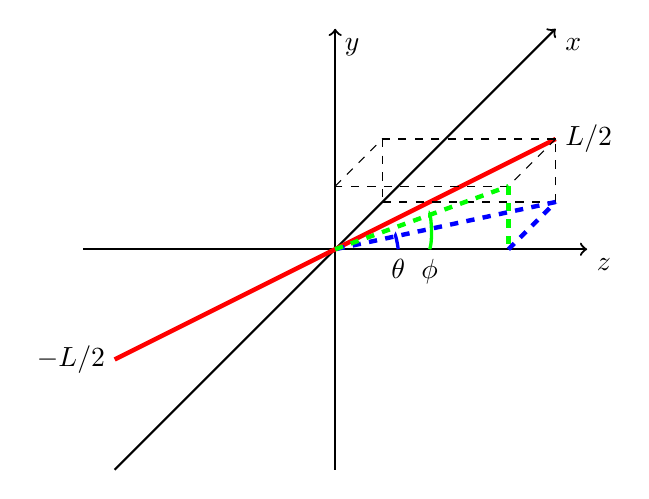
\begin{tikzpicture}[scale=0.4]
	%
	\draw [thick, ->] (-8,0) -- (8,0);
	\draw [thick, ->] (0,-7) -- (0,7);
	\draw [thick, ->] (-7,-7) -- (7,7);
	\draw [red, ultra thick] (-7,-3.5) -- (7,3.5);
	\node [below right] at (8,0) {$z$};
	\node [below right] at (0,7) {$y$};
	\node [below right] at (7,7) {$x$};
	\node [right] at (7.0,3.5) {$L/2$};
	\node [left] at (-7.0,-3.5) {$-L/2$};
	%
	\draw [dashed] (7, 3.5) -- (5.5, 2.0);
	\draw [green, ultra thick, dashed] (5.5, 2.0) -- (5.5, 0.0);
	\draw [blue, ultra thick, dashed] (5.5, 0.0) -- (7.0, 1.5);
	\draw [dashed] (7.0, 1.5) -- (7.0, 3.5);
	\draw [dashed] (7.0, 3.5) -- (1.5, 3.5);
	\draw [dashed] (5.5, 2.0) -- (0.0, 2.0);
	\draw [dashed] (0.0, 2.0) -- (1.5, 3.5);
	\draw [dashed] (1.5, 3.5) -- (1.5, 1.5);
	\draw [dashed] (1.5, 1.5) -- (7.0, 1.5);
	\draw [blue, ultra thick, dashed] (7.0, 1.5) -- (0.0, 0.0);
	\draw [green, ultra thick, dashed] (0.0, 0.0) -- (5.5,2.0);
	%
	\draw[blue, very thick] (1.9,0.4) to [out=90,in=95] (2.0,0.0);
	\draw[green, very thick] (3.0,1.0) to [out=90,in=70] (3.0,0.0);
	%
	\node [below] at (2.0,0.0) {${\theta}$};
	\node [below] at (3.0,0.0) {${\phi}$};
	\end{tikzpicture}
	\caption{Wire centered (red) at the origin including the angles $\phi$ and $\theta$ as defined for the directional cosines in Eqn.~\ref{wire:eqn:3}.\label{wire:fig:2}}
\end{figure}

In case the wire lies parallel to the longitudinal axis ($\phi=\theta=0$), the transverse potential $A_{x,y}$ vanish and the longitudinal potential can be further simplified, leading to:
\begin{align}\label{wire:eqn:4}
A_x(x,y,z)&=0 \nonumber\\
A_y(x,y,z)&=0 \nonumber\\
A_z(x,y,z)&=\frac{I\mu_0}{4\pi}\cdot\left(\asinh\left(\frac{L/2-z}{\sqrt{x^2+y^2}}\right)-\asinh\left(\frac{-L/2-z}{\sqrt{x^2+y^2}}\right)\right)
\end{align}  
The Hamiltonian for the wire is then simply $H=-A_s=-A_z$. 

The kick experienced by an arbitrary particle with coordinates $(x,y,z)$ using a first order symplectic integrator is then given by:
\begin{align}\label{wire:eqn:5}
\Delta p_x &= \int\limits_{-L_{\mathrm{emb}}/2}^{+L_{\mathrm{emb}}/2}{\frac{\partial A_z(x,y,s)}{\partial x}ds}, \\
 \Delta p_y & = \int\limits_{-L_{\mathrm{emb}}/2}^{+L_{\mathrm{emb}}/2}{\frac{\partial A_z(x,y,s)}{\partial y}ds},\\
 \Delta x &=\Delta y=\Delta \delta = \Delta \sigma = 0 
\end{align}
where $L_{\mathrm{emb}}$ is the embedding drift or integration length (see Fig.~\ref{wire:fig:1}), which takes into account the fringe field of the wire, while the parameter $L$ in Eqn.~\ref{wire:eqn:4} denotes the physical length of the wire. A symplectic rotation of the coordinate system as described in \cite{forest99} is included in order to compute the transport map for arbitrary orientation, explicitly arbitrary angles $\theta$ and $\phi$ in Fig.~\ref{wire:fig:2}.  

The first order symplectic transport map in thin lens approximation for an arbitrary orientation of the wire can then be obtained by the following steps:

\begin{description}
\item[Step 1] Shift to the origin: We define the new variables
	\begin{align}
	r_x &:= x -x_{co}  + dx \nonumber\\
	r_y &:= y -y_{co} + dy
	\end{align}
where $x_{co}$ and $y_{co}$ denotes the closed orbit at the center of the wire.

\item[Step 2] Symplectic rotation in $(x,z)$ by $\theta$ as described in \cite{forest99}: In a drift space the normalized momenta $p_i$ are related by $p_x^2+p_y^2 +p_z^2=(1+\delta)^2$  and we can thus write $p_z$ as
\begin{align}
p_z = \sqrt{(1+\delta)^2-p_x^2-p_y^2}
\end{align}
The rotation by $\theta$ can then be expressed as a rotation first in $(p_x,p_z)$:
 \begin{align}
 p_x & \to   p_x \cdot \cos \theta + p_z \cdot \sin\theta \nonumber\\
 p_z & \to - p_x \cdot \sin \theta + p_z \cdot \cos\theta
 \end{align}
 followed by a transformation in $(r_x,r_y)$:
 \begin{align}
 r_x & \to r_x \left(\cos\theta - \frac{p_x}{p_z} \cdot \sin\theta\right)  \nonumber\\
 r_y & \to r_y - r_x \cdot\frac{p_y}{p_z}\cdot\sin\theta  
 \end{align}

\item[Step 3] Symplectic rotation in $(y,z)$ by $\phi$ as described in \cite{forest99}: The new $p_z$ is again defined as
$p_z = \sqrt{(1+\delta)^2-p_x^2-p_y^2}$ using the updated values of $p_x,p_y$ from Step 2. Analogical to the symplectic rotation in $(x,z)$, the rotation by $\phi$ in $(y,z)$ can be expressed as a rotation first in $(p_y,p_z)$:
\begin{align}
p_y & \to   p_y \cdot\cos \phi + p_z \cdot\sin\phi \nonumber\\
p_z & \to - p_y \cdot\sin \phi + p_z \cdot\cos\phi
\end{align}
followed by a transformation in $(r_x,r_y)$:
\begin{align}
r_x & \to r_x - r_y \cdot\frac{p_x}{p_z}\cdot\sin\phi \nonumber\\ 
r_y & \to r_y \left(\cos\theta - \frac{p_y}{p_z} \sin\theta\right)
\end{align}

\item[Step 4] Application of the symplectic kick of a wire aligned along the longitudinal axis ($\theta=\phi=0$): We define the radius $r$ in the $(r_x,r_y)$ by:
  \begin{align}
  r^2:=r_x^2+r_y^2
  \end{align}
The thin lens kick of the wire aligned along the longitudinal axis can then be expressed by:
 \begin{align}
 p_x & \to p_x - 10^{-7}\cdot I \frac{e}{P_0}\frac{r_x}{r^2} \left(d^+-d^- \right) - p_{co,wire} \nonumber\\
 p_y & \to p_y - 10^{-7}\cdot I \frac{e}{P_0}\frac{r_y}{r^2} \left(d^+-d^- \right) -p_{co,wire} 
 \end{align}
with $d^+$ and $d^-$ defined as:
 \begin{align}
d^+&=\sqrt{(L_{\mathrm{emb}}+L)^2+4r^2}\\
d^-&=\sqrt{(L_{\mathrm{emb}}-L)^2+4r^2}
 \end{align}
As reminder $L$ denotes the physical length of the wire and $L_{\mathrm{emb}}$ the length of the embedded drift. The parameter $p_{co,wire}$ is the closed orbit kick due to the wire. This kick is only subtracted if \emph{ibeco} is equal to $1$ in the BEAM block.

\item[Step 5] Backward rotation by $-\phi$ in $(p_y,p_z)$: The new $p_z$ is again defined as
$p_z = \sqrt{(1+\delta)^2-p_x^2-p_y^2}$ using the updated values of $p_x,p_y$ from Step 4. The rotation is then given by:
\begin{align}
p_y & \to   p_y \cdot \cos \phi - p_z \cdot \sin\phi \nonumber\\
p_z & \to   p_y \cdot \sin \phi + p_z \cdot \cos\phi 
\end{align}
\item[Step 6] Backward rotation by $-\theta$ in $(p_x,p_z)$: The new $p_z$ is again defined as
$p_z = \sqrt{(1+\delta)^2-p_x^2-p_y^2}$ using the updated values of $p_x,p_y$ from Step 5. The rotation is then given by:
\begin{align}
 p_x & \to   p_x \cdot \cos \theta - p_z \cdot \sin\theta \nonumber\\
 p_z & \to   p_x \cdot \sin \theta + p_z \cdot \cos\theta 
\end{align}
\end{description}
Note that as required for a thin lens approximation, the map does not change $x$ and $y$.

\subsection{Crab cavity}
The voltage of the crab cavity is denoted by $V$, the frequency by $f$ and the phase by $\phi$. The map for a horizontal
crab cavity is
\begin{align}
    p_x \to p_x - \frac{V}{p}\cdot(1+\delta) \sin\left(2\pi f\frac{\sigma}{c}+\phi \right) \\
    \delta \to \delta - 2\pi f \frac{V}{pc}\cdot x \cdot \cos\left(2\pi f \frac{\sigma}{c}+\phi\right).
\end{align}
Followed by updates of the momentum and energy due to the change of $\delta$. The map for a vertical crab cavity
is given by replacing $x\to y$ and $p_x\to p_y$ in the map above.

\subsection{AC-dipole}
The excitation amplitude of the AC-dipole is denoted by $A$ [Tm], the excitation frequency by $q_d$ [$2\pi$] and the phase of the excitation by $\phi$. The map
presented here is for a purely horizontal dipole, the map for a vertical dipole is obtained by replacing $p_x\to p_y$.

The effect of the AC-dipole is split into four stages. The turn number is denoted by $n$.
\begin{enumerate}
  \item A number of free turns $n_{\text{free}}$, in which the AC-dipole has no effect on the motion.
  \item Ramp-up of the voltage from $0$ to the excitation amplitude $A$ for $n_{\text{ramp-up}}$ turns.
        \begin{align}
            n' &= \frac{n-n_{\text{free}}}{n_{\text{ramp-up}}} \\
            p_x &\to p_x + n' \cdot \frac{A}{pc} \cdot(1+\delta) \sin\left(2\pi q_d\cdot(n-n_{\text{free}})+\phi\right)
        \end{align}
  \item Constant excitation amplitude for $n_{\text{flat}}$ turns.
        \begin{align}
            p_x &\to p_x + \frac{A}{pc}\cdot(1+\delta)\sin\left(2\pi q_d\cdot(n-n_{\text{free}})+\phi\right)
        \end{align}
  \item Ramp-down of the voltage from the excitation amplitude $A$ to $0$ for $n_{\text{ramp-down}}$ turns.
        \begin{align}
            n' &= \frac{n-n_{\text{free}}-n_{\text{ramp-up}}-n_{\text{flat}}-n_{\text{ramp-down}}}{n_{\text{ramp-down}}} \\
            p_x &\to p_x + n' \cdot \frac{A}{p} \cdot(1+\delta) \sin\left(2\pi q_d\cdot(n-n_{\text{free}})+\phi\right)
        \end{align}
\end{enumerate}

\subsection{Electron lens}
\label{elense}
Electron lenses are devices where the tracked beam interacts with a beam of electrons. The electron beam travels co--axial to the main beam; it
is contained in a thick cylinder of inner radius $R_1$ and outer radius $R_2$.
If $R_1>0$, then the lens is hollow. The interaction is purely via the Lorentz
force. These devices can be used for compensating beam--beam effects or as
collimation devices~\cite{Shiltsev:2112966}.

The implementation in SixTrack does not start from the Hamiltonian but from the
integration of the Lorentz force along the length of the e--lens in idealised
conditions. The e--lens \emph{must be a thin lens};
the derivation of the kick assumes electrons moving along straight paths,
parallel to the beam, for an indefinite length, and an axis--symmetric
transverse distribution (cylindrical symmetry). Hence,
the derivation of the kicks and the implemented tracking is developed in cylindrical coordinates, where
\begin{equation}
  r=\sqrt{x^2+y^2}
\end{equation}
is the radial coordinate used to compute the kick. Moreover,
the implementation of the hollow e--lens has no explicit dependence on the
beam energy, taken into account only in the form of the input parameter
$\theta_{\rm max}$ provided by the user. Moreover, a change of the particle
energy could occur if the particle enters with an initial $x'$ or
$y'$ and thus sees an accelerating or decelerating field. These effects
are not taken into account for the time being.

The implementation in SixTrack is very similar to the one in
Merlin~\cite{HReLens}. There you can also find a complete derivation of
the equations laid down in the following.

\subsubsection{Treatment of the Kick}
The kick received by a beam particle can be conveniently described as:
\begin{equation}
  \theta(r)=\frac{f(r)}{r/R_2} \theta_{\rm R_2}
  \label{elense:eqn:0}
\end{equation}
where $\theta_{\rm R_2}$ is the kick imparted by the electron beam when the beam particle
is at $r=R_2$ and $f(r)$ is a shape function which depends on the radial distribution of the
electron beam.
$\theta_{\rm R_2}$ reads like
\begin{equation}
\theta_{\rm R_2} = \frac{LI_T(1\pm\beta_e\beta_b)}{2\pi\epsilon_0  \left(B\rho\right)_b\beta_e\beta_b c^2}\cdot\frac{1}{R_2}
\end{equation}
where $L$ is the length of the e--lens, $I_T$ the total electron beam current, $\beta_{e}$ and $\beta_{b}$ the relativistic $\beta$ of electron and tracked beam, $(B\rho)|_b$ the magnetic rigidity of the beam (synchronous particle), $c$ the speed of light and $\epsilon_0$ the vacuum permittivity. The $\pm$-sign represents the two cases of the electron beam travelling in the direction of the tracked beam ($v_e v_b>0$) leading to ``$-$" or in the opposite direction ($v_e v_b<0$) leading to ``$+$". For hollow electron beam collimation, electron and tracked beam travel in opposite directions. It should be noted that $\theta_{\rm R_2}$ depends on the magnetic rigidity $(B\rho)_b$ of the tracked beam and thus on the beam momentum; hence, during tracking, the actual magnetic rigidity of each beam particle and its charge--to--mass ration is taken into account when computing the kick to be imparted.

$f(r)$ reads like
\begin{equation}
  f(r) = \frac{I(r)}{I_T}=\frac{2\pi}{I_T}\int_{0}^r r\rho(r) \mathrm{d}r,
  \label{elense:eqn:1}
\end{equation}
where $I(r)$ is the current enclosed in a radius
$r$ and $\rho(r)$ is the electron beam density distribution. Taking into account the
cylindrical symmetry of the electron distribution and the fact that the electron
distribution is contained in a cylinder $R_1<r<R_2$, $f(r)$ can be split into
three expressions based on respective domains as follows
\begin{equation}
f(r) =
\begin{cases} 0 &,\quad r \leq R_1\\
\tilde f(r) &,\quad R_1 < r < R_2\\
1 &,\quad R_2 \leq r
\end{cases}
\label{elense:eqn:5}
\end{equation}
where $\tilde f(r)$ changes functional shape according to the transverse
distribution to be simulated.

Using Eq.~\ref{elense:eqn:0}, the kick in $(x',y')$ can then be expressed as
\begin{align}
x'&=x'-\frac{x}{r}\;\frac{f(r)}{r/R_2}\;\theta_{\rm R_2}\frac{\chi}{1+\delta}\label{elense:eqn:2}\\
y'&=y'-\frac{y}{r}\;\frac{f(r)}{r/R_2}\;\theta_{\rm R_2}\frac{\chi}{1+\delta}\label{elense:eqn:3}
\end{align}
where $\frac{x}{r}=\cos(\phi)$ and $\frac{y}{r}=\sin(\phi)$ allow to get the
horizontal and vertical kicks from the radial one.
Off-momentum particles and different ion species are taken into
account via the factor $\chi/(1+\delta)$, which comes from the definition of
magnetic rigidity of ion species different from the nominal one
($B\rho|_b$) given by
\begin{equation}
  B\rho = B\rho|_b \frac{1+\delta}{\chi},
\end{equation}
where $\chi$ is the charge--over--mass ratio of the tracked and synchronous
particles, i.e.~$\chi=(q/m)/(q_0/m_0)$ and $\delta$ is the one used in case of
multi--isotop tracking, i.e.~$\frac{(p/m)}{p_0/m_0}-1$~\cite{Hermes:2241364};
hence, the current implementation of
e--lenses is compatible with ion tracking.

If the electron lens is centred around $(x_{\rm offset},y_{\rm offset})$
(local reference frame), particle coordinates $(x,y)$ are simply transformed
into:
\begin{align}
\tilde x&\rightarrow x-x_{\rm offset}\\
\tilde y&\rightarrow y-y_{\rm offset}\\
\end{align}
before computing the radial position, without touching the above processing.

\subsubsection{Uniform electron profile}
The uniform distribution of the electron beam between $R_1$ and $R_2$
can be described as:
\begin{equation}
\rho(r) = \frac{I_T}{\pi (R_2^2 -R_1^2) } \quad R_1 < r < R_2
\end{equation}
This leads the middle term of $f(r)$ (see Eq.~\ref{elense:eqn:1}) to be:
\begin{equation}
\tilde f(r)=\frac{r^2-R_1^2}{R_2^2-R_1^2}
\end{equation}

\subsubsection{Gaussian electron profile}
The Gaussian distribution of the electron beam between $R_1$ and $R_2$
can be described as:
\begin{equation}
\rho(r) = \frac{I_T \exp\left[-\frac{r^2}{2\sigma^2}\right]}{2\pi\sigma^2} \quad R_1 < r < R_2
\end{equation}
This leads the middle term of $f(r)$ (see Eq.~\ref{elense:eqn:1}) to be:
\begin{equation}
  \tilde f(r)=\frac{\exp\left[-\frac{R_1^2}{2\sigma^2}\right]-\exp\left[-\frac{r^2}{2\sigma^2}\right]}
                   {\exp\left[-\frac{R_1^2}{2\sigma^2}\right]-\exp\left[-\frac{R_2^2}{2\sigma^2}\right]}
  \label{elense:eqn:4}
\end{equation}
The denominator in Eq.~\ref{elense:eqn:4}, which is added after integrating
the Gaussian profile as in Eq.~\ref{elense:eqn:1}, is a normalisation factor
necessary to have $\tilde f(R_2)=1$. Hence, the same factor must be considered
in the expression of $\theta_{\rm R_2}$, which then becomes
\begin{equation}
  \theta_{\rm R_2} = \frac{LI_T(1\pm\beta_e\beta_b)}{2\pi\epsilon_0  \left(B\rho\right)_b\beta_e\beta_b c^2}\cdot\frac{1}{R_2}
  \cdot\left\{\exp\left[-\frac{R_1^2}{2\sigma^2}\right]-\exp\left[-\frac{R_2^2}{2\sigma^2}\right]\right\}
\end{equation}
It should be noted that, contrary to the case of the uniform distribution,
$\theta_{\rm R_2}$ does not coincide with the highest kick; the highest kick is
found only at:
\begin{equation}
  \frac{\textrm{d}f}{\textrm{d}r}=0
\end{equation}
which leads to the following equation
\begin{equation}
  \exp\left[-\frac{r^2}{2\sigma^2}\right] = \frac{\exp\left[-\frac{R_1^2}{2\sigma^2}\right]}{r^2+\sigma^2},
\end{equation}
that can be solved graphically or numerically, not analitically.

\subsection{Misalignment}

Misalignments of elements affects the coordinates at the entrance of an
element as follows
\begin{align}
    x &\to (x-x_s)\cdot t_c + (y-y_s)\cdot t_s \\
    y &\to -(x-x_s)\cdot t_s + (y-y_s)\cdot t_c,
\end{align}
where $x_s$ and $y_s$ are the displacements in the horizontal and vertical
directions, respectively. $t_c$ and $t_s$ are the cosine and sine of the tilt
angle for the element.

\section{Optics calculations}
\label{opt}
Optics calculation are needed to study the motion around the closed orbit. By defining $z$ as the vector of $2 k$ coordinates,  
\begin{align}\label{opt:eqn:1}
z&=(z_1,\ldots,z_{2k})^T=(x-x_0,p_x-p_{x0},y-y_0,p_y-p_{y0},\tau-\tau_0,p_t-p_{t0})^T
\end{align}
one can define linear transfer maps (e.g. $M_{1\to 2}$ that propagates coordinates between two points $s_1$, $s_2$) and the one-turn map (e.g. $M_1$ that combines the effects for one turn starting from $s_1$):
\begin{align}\label{opt:eqn:2}
z(s_2)&= M_{1\to 2} z(s_1) & z(C+s_1) &= M_1 z(s_1).
\end{align}
In the following we will describe the optics calculation based on the Ripken formalism described in \cite{willeke88}. A good summary is also given in the MAD8 physics manual \cite{mad8phys}.

\subsection{Diagonalisation of one-turn matrix}
\label{opt:sec:1}
Since the matrices derive from symplectic maps, the eigenvalue spectrum of the one-turn map $M$ consists of 2$k$ distinct eigenvalues and linearly independent eigenvectors. In addition, for the motion to be stable the eigenvalues $\lambda_k^{\pm}$ with eigenvectors $v_k^{\pm}$ have to be complex \cite{willeke88}:
\begin{align}
M v_k^\pm  =  \lambda_k^\pm v_k^\pm, \ k=1,\ldots, 3 \\
v_k^+=(v_k^-)^*, \quad \lambda_k^+=(\lambda_k^-)^*, \quad |\lambda_k^{\pm}|=1
\end{align}
As the eigenvectors are linearly independent $M$ can be diagonalized with
\begin{align}
M &= V \Lambda V^{-1},
\end{align}
where $V$ consists of the eigenvectors and $\Lambda$ of the eigenvalues:
\begin{align}
V=&\left(
\begin{array}{cccc}
v^+_{1,1} & v^-_{1,1} & \cdots & v^-_{3,1}\\
v^+_{1,2} & v^-_{1,2} & \cdots & v^-_{3,2}\\
\vdots    & \vdots    & \vdots & \vdots \\
\end{array}
\right)  &
\Lambda=&\left(
\begin{array}{cccc}
\lambda^+_1 &    & &\\
& \lambda^-_1 & &\\
& & \ddots & \\
& & & \lambda^-_3
\end{array}
\right)
\end{align}
for which $v^{\pm}_{i,j}$ is the component $j$ of eigenvector $v_i^{\pm}$.

The same calculation can be carried out with real numbers by the following definitions:
\begin{align}\
v_k^\pm &= a_k\pm ib_k, & \lambda_k^\pm &= \cos \mu_k \pm i \sin \mu_k, &
\mu_k, a_k, b_k \in \mathbb{R}
\end{align}
such that:
\begin{align}\label{opt:eqn:1:1}
M=&W R W^{-1}
\end{align}
with
\begin{align}
R=R(\mu_k)=&\left(
\begin{array}{ccccc}
\cos \mu_1 & \sin \mu_1  &  & &\\
-\sin \mu_1 & \cos \mu_1 &  & &\\
&    & \ddots & &\\
& & & \cos \mu_3 & \sin \mu_3 \\
& & & -\sin \mu_3 & \cos \mu_3 \\
\end{array}
\right), \\
W=&\left(
\begin{array}{ccccc}
a_{1,1} & b_{1,1} & \cdots & a_{3,1} & b_{3,1} \\
a_{1,2} & b_{1,2} & \cdots & a_{3,2} & b_{3,2} \\
\vdots    & \vdots    & \vdots & \vdots\\
a_{1,6} & b_{1,6} & \cdots & a_{3,6} & b_{3,6} \\
\end{array}
\right)
\end{align}
Usually $\mu_k$ is written as $\mu_k=2\pi Q_k$, where $Q_k$ is then the tune of the mode $k$.
\subsection{Normalisation of eigenvectors}
\label{opt:sec:2}
By convention, the eigenvectors and values are normalized, sorted and rotated so that the following three conditions are fulfilled:
\begin{enumerate}
\item Plane 1 is associated with the horizontal, plane 2 with the vertical and plane 3 with the longitudinal plane. This is achieved by first normalizing the eigenvectors $v_k^{\pm}$ and then sorting them so that:
\begin{align}\label{opt:eqn:2:1}
|v_{j,2j-1}^{+}| =|v_{j,2j-1}^{-}| = \max_{k=1,2,3} v_{k,j}, \quad j=1,\ldots, 3
\end{align}
\item The eigenvectors are then rotated with a phase term $\psi_k$
\begin{align}
v_k& \to v_k \exp(i \psi_k) 
\end{align}
such that
\begin{align}\label{opt:eqn:2:2}
\mathrm{angle}(v_{k,2k-1}^{+})=0 \leftrightarrow \psi_k=-\mathrm{angle}(v_{k,2k-1}^{+})
\end{align}
In real space, Eqn.~\ref{opt:eqn:2:1} and \ref{opt:eqn:2:2} then become equivalent to:
\begin{align}
|a_{j,2j-1}| &=\max_{k=1,2,3} |a_{k,j}|,& b_{j,2 j-1}&=0, & j=1,\ldots, 3
\end{align}
This has the effect that a particle with $x=0$ is transformed to $\tilde x$ in the normalized phase space.
\item The sign of $b_{k,j}$ is fixed by the symplectic condition on $W$
\begin{align}
W^T S W = S
\end{align}
with $S$ defined as
\begin{align}
S&=\left(
\begin{array}{ccc}
0 & 1  &  \\
-1 & 0  &  \\
&    & \ddots \\
\end{array} 
\right)
\end{align}
which is equivalent to:
\begin{align}\label{opt:eqn:2:3}
a_k^T \cdot S \cdot b_k &=1, \quad b_k^T \cdot S \cdot a_k =-1, & \text{ for } k=l\nonumber\\
a_k^T \cdot S \cdot b_l &=0, & \text{ for }  k\not=l\\
a_k^T \cdot S \cdot a_l &=0, \quad b_k^T \cdot S \cdot b_l =0,  & k,l=1,\ldots,3 \nonumber
\end{align}
Eqn.~\ref{opt:eqn:2:3} yields that in phase space $a_k$ is thus obtained by an anticlockwise rotation of $b_k$ by $\pi/2$ and a scaling of its length with $|a_k|=\frac{1}{|b_k|}$.
\end{enumerate}
\subsection{Conversion to normalized coordinates}
\label{opt:sec:3}
We will show in the following that in the normalized phase space the propagation of particle coordinates $z(s)$ from $s_1$ to $s_2$ is just a rotation by an angle $\phi_k$ in the $k=1,\ldots,3$ planes, while the amplitude $I_k$ and initial phase $\phi_{k,0}$ stay constant, explicitly $z(s)$ is then given by:
\begin{align}\label{opt:eqn:3:3}
z(s)=\sum_{k=1}^3 \sqrt{2I_k}\left(
a_k(s) \cos \left(\phi_{k,0} + \phi_k(s)\right) -
b_k(s) \sin \left(\phi_{k,0} + \phi_k(s)\right)
\right) 
\end{align}
and
\begin{align}
z(s_2)&=W(s_2)R(\phi_k)W(s_1)^{-1}z(s_1), \\
&\hspace{30pt} \text{ with } \phi_k=\phi_k(s_2)-\phi_k(s_1)\nonumber
\end{align}
This implies that one turn is simply a rotation by $\phi_k=2\pi Q_k$ where $Q_k$ is the tune of the mode $k$. In the transverse plane the tune ($Q_{I,II}$) is usually positive and the particles rotate clockwise, while in the longitudinal plane the tune ($Q_{III}$) is negative above $\gamma_T$ leading to an anticlockwise rotation.

For the derivation the following steps are needed:
\begin{enumerate}
\item The effect of one turn on the normalized variable $\tilde z(s)=W^{-1}(s) z(s)$ is a rotation:
\begin{align}\label{opt:eqn:3:1}
\tilde z(C+s) = W^{-1}z(s+C)\overset{(\rm Eqn.\ref{opt:eqn:1:1})}{=}W^{-1}WRW^{-1}z(s)= R\tilde z(s),
\end{align}
As $M$ and $R$ are symplectic also $W$ is symplectic, and its inverse is thus given by $S^{-1}W^{T}S$, explicitly:
\begin{align}
W^{-1}&=
\left(
\begin{array}{cccccc}
b_{12} & - b_{11} &   b_{14} & - b_{13} &   b_{16} & - b_{15}\\
- a_{12} &   a_{11} & - a_{14} &   a_{13} & - a_{16} &   a_{15}\\
b_{22} & - b_{21} &   b_{24} & - b_{23} &   b_{26} & - b_{25}\\
- a_{22} &   a_{21} & - a_{24} &   a_{23} & - a_{26} &   a_{25}\\
b_{32} & - b_{31} &   b_{34} & - b_{33} &   b_{36} & - b_{35}\\
- a_{32} &   a_{31} & - a_{34} &   a_{33} & - a_{36} &   a_{35}\\
\end{array}
\right)
\end{align}
\item The one-turn map and $W$-matrix can be propagated from $s_1$ to $s_2$ by
\begin{align}
M_2&=M_{1 \to 2} M_1 M^{-1}_{1 \to 2}  &
W_2&=M_{1 \to 2} W_1
\end{align}
As Eqn.~\ref{opt:eqn:3:1} represents a similarity transformation, the eigenvalues are thus independent of the position $s$ and as the rotation matrix $R$ consists of the eigenvalues of $M$, the angle of the rotation $\mu_k=2\pi Q_k$ is thus also independent of $s$.

\item As Eqn.~\ref{opt:eqn:1:1} represents a basis transformation from the standard $\mathbb{R}^2$ basis to the eigenvector basis, the vectors $a_k$ and $b_k$ are projected onto (Eqn.~\ref{opt:eqn:2:3}):
\begin{align}\label{opt:eqn:3:2}
\tilde a_1=W^{-1}a_1&=-SW^TSa_1\nonumber\\
&=-S(a_1Sa_1,b_1Sa_1,\ldots,b_3Sa_1)^T=(1,0,\ldots,0)\nonumber\\
\tilde b_1=W^{-1}b_1&=-SW^TSb_1\nonumber\\
&=-S(a_1Sb_1,b_1Sb_1,\ldots,b_3Sb_1)^T=(0,1,\ldots,0)\\
\cdots & \nonumber\\
\tilde b_3=W^{-1}b_3&=-SW^TSb_3\nonumber\\
&=-S(a_1Sb_3,b_1Sb_3,\ldots,b_3Sb_3)^T=(0,0,\ldots,1)\nonumber
\end{align}
in the normalized phase space.
\item From Eqn.~\ref{opt:eqn:3:1} it follows that the amplitude $I_k$ and initial phase $\phi_{k0}$ of $\tilde z=W^{-1}z=(\tilde z_{a_1},\tilde z_{b_1},\ldots,\tilde z_{b_3})$ 
\begin{align}
I_k&=\frac{(\tilde z_{a_k})^2 +(\tilde z_{b_k})^2}{2}, \quad k=1,\ldots,3\label{opt:eqn:20a}\\
\tan\phi_{k0}&=-\frac{\tilde z_{b_k}}{\tilde z_{a_k}} \label{opt:eqn:20b}
\end{align}
are constants of the motion, which is illustrated in Fig.~\ref{opt:fig:1}.
\begin{figure}[h]
	\centering
	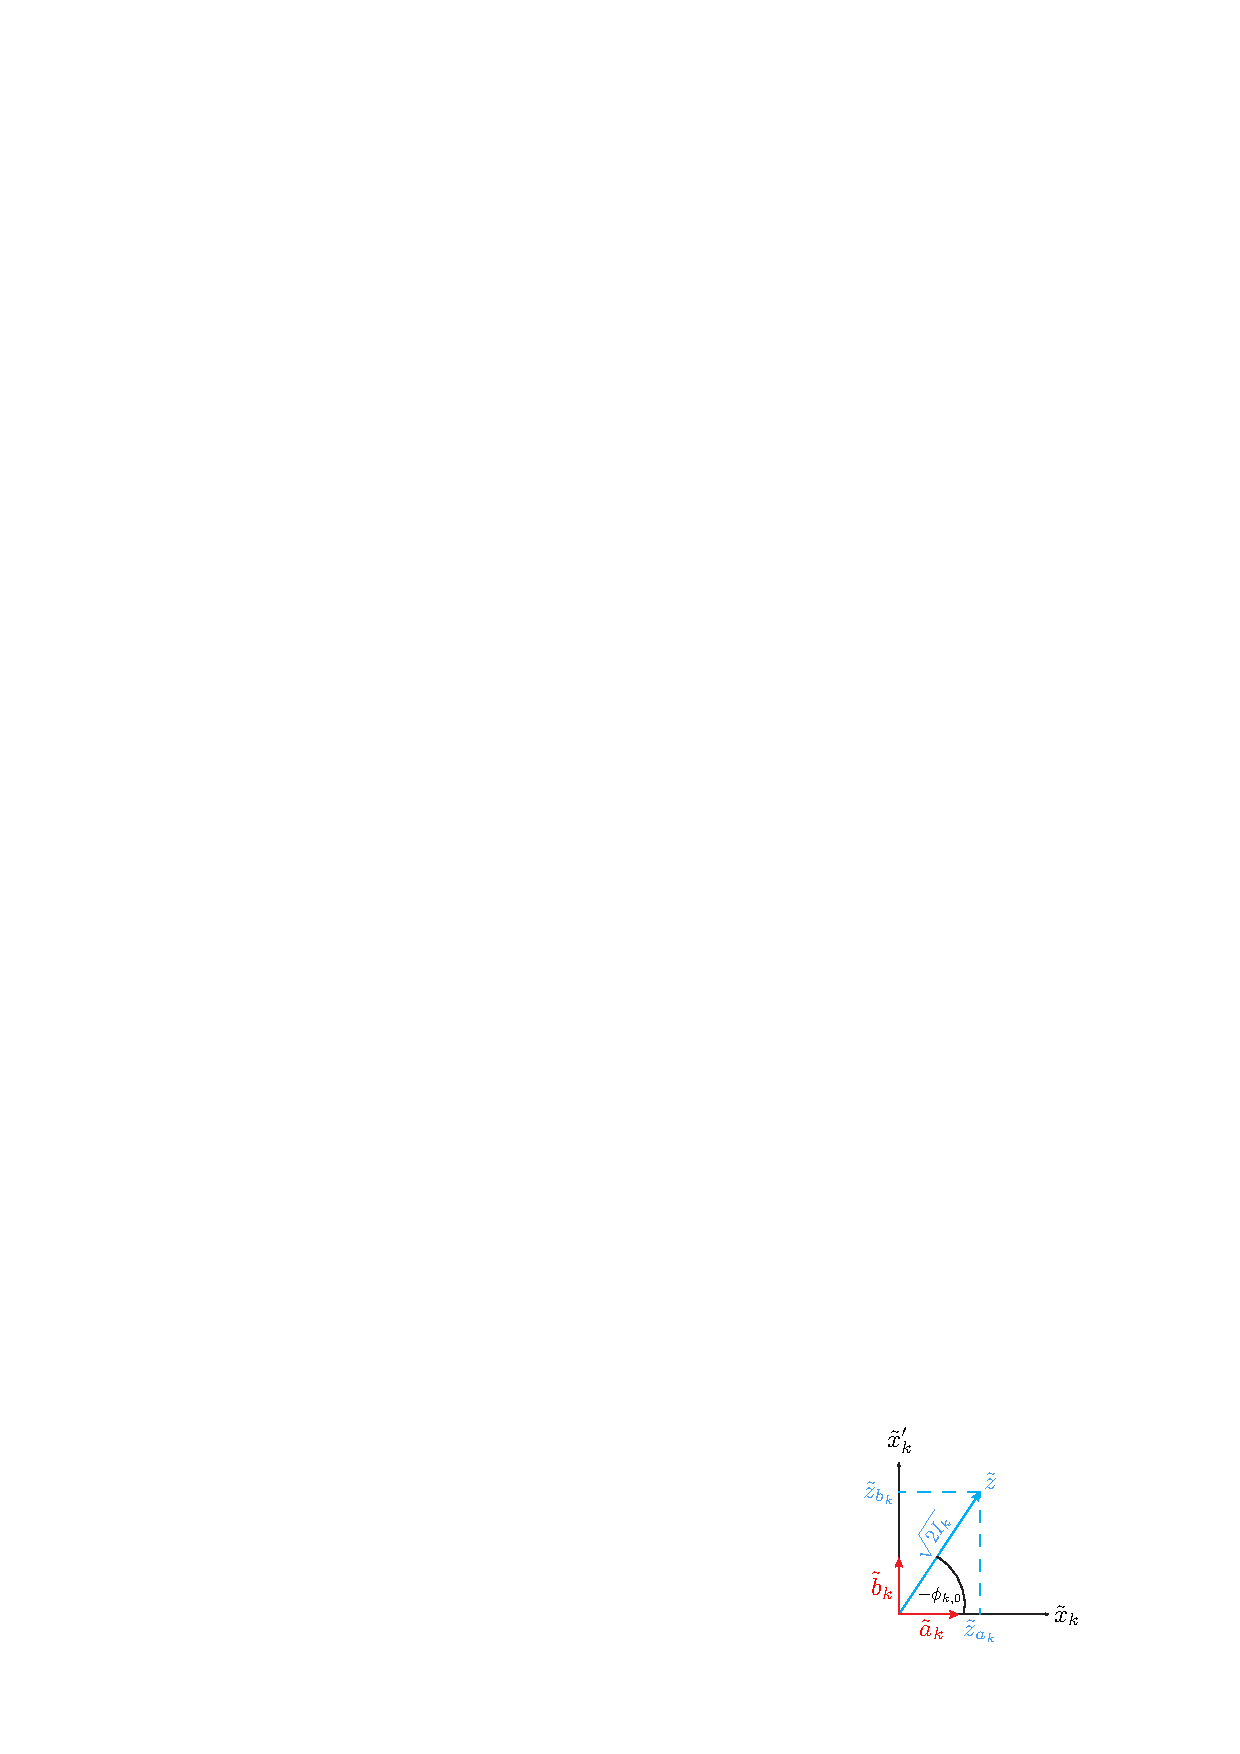
\includegraphics{normalized_phase_space_cropped.pdf}
	\caption{Normalized phase space.\label{opt:fig:1}}
\end{figure}
The initial phase is defined with a minus sign in view of the definition of the Twiss parameters, where the initial phase is then added (and not subtracted) to the phase advance. The components of $\tilde z$ are then explicitly given by:
\begin{align}
\tilde z_{a_k}&= \sum_{j=1}^3  b_{k,2j} z_{2j-1}- b_{k,2j-1} z_{2j}, \quad k=1,\ldots,3\\
\tilde z_{b_k}&= \sum_{j=1}^3 a_{k,2j-1} z_{2j}- a_{k,2j} z_{2j-1}, \quad k=1,\ldots,3.
\end{align}
An arbitrary vector $z(s)$ can thus be written in the following form:
\begin{align}
 z(s)&=W(s)\tilde z(s)\nonumber\\
 &=W(s)\left(\sum_{k=1}^{3}\tilde z_{a_k}\tilde a_k + \tilde z_{b_k}\tilde b_k\right)\nonumber\\
 &=\sum_{k=1}^{3}\tilde z_{a_k}W(s)\tilde a_k + \tilde z_{b_k}W(s)\tilde b_k\overset{\rm Eqn.~\ref{opt:eqn:3:2}}{=}\sum_{k=1}^{3}\tilde z_{a_k}a_k + \tilde z_{b_k}b_k\nonumber\\
 &\overset{\rm Eqns.~\ref
 	{opt:eqn:20a},\ref{opt:eqn:20b}}=\sum_{k=1}^{3}\sqrt{2I_k}\left(a_k\cos{\phi_{k0}}-b_k\sin{\phi_{k0}}\right)
\end{align}
\end{enumerate}

\subsection{Twiss parameters}
\label{opt:sec:4}
In the following the parameter $k$ will always be used for the mode $k$ and the parameter $j=1,2,3$ for the horizontal ($x,x'$), vertical ($y,y'$) and longitudinal plane $(\sigma,\delta)$ in the phase space. $z_{2j-1}$ then stands for the coordinates $(x,y,\sigma$) and $z_{2j}$ for $(x',y',\delta$).

The Twiss parameters can be introduced by writing the components of the eigenvector basis $(a_k(s),b_k(s))$ as the product of two envelope functions $\sqrt{\beta_{k,j}(s)}$, $\sqrt{\gamma_{k,j}(s)}$ and phase functions $\phi_{k,j}(s)$, $\bar\phi_{k,j}(s)$, also called Twiss parameters or lattice functions, with
\begin{align}
a_{k,2j-1}(s)&=\sqrt{\beta_{k,j}(s)}\cos{\phi_{k,j}(s)},\nonumber\\ b_{k,2j-1}(s)&=\sqrt{\beta_{k,j}(s)}\sin{\phi_{k,j}(s)}, \ k,j=1,\ldots,3, \label{opt:eqn:4:1}\\
a_{k,2j}(s)&=\sqrt{\gamma_{k,j}(s)}\cos{\bar\phi_{k,j}(s)}, \nonumber\\
b_{k,2j}(s)&=\sqrt{\gamma_{k,j}(s)}\sin{\bar\phi_{k,j}(s)}, \ k,j=1,\ldots,3 \label{opt:eqn:4:2}
\end{align}
where $\beta_{k,j}(s), \alpha_{k,j}(s), \gamma_{k,j}(s)$ represent the projection of the ellipse of mode $k$ on the plane of coordinates $z_{2k-1}-z_{2k}$ (see Fig.~\ref{opt:fig:2})
\begin{figure}[!ht]
	\centering
	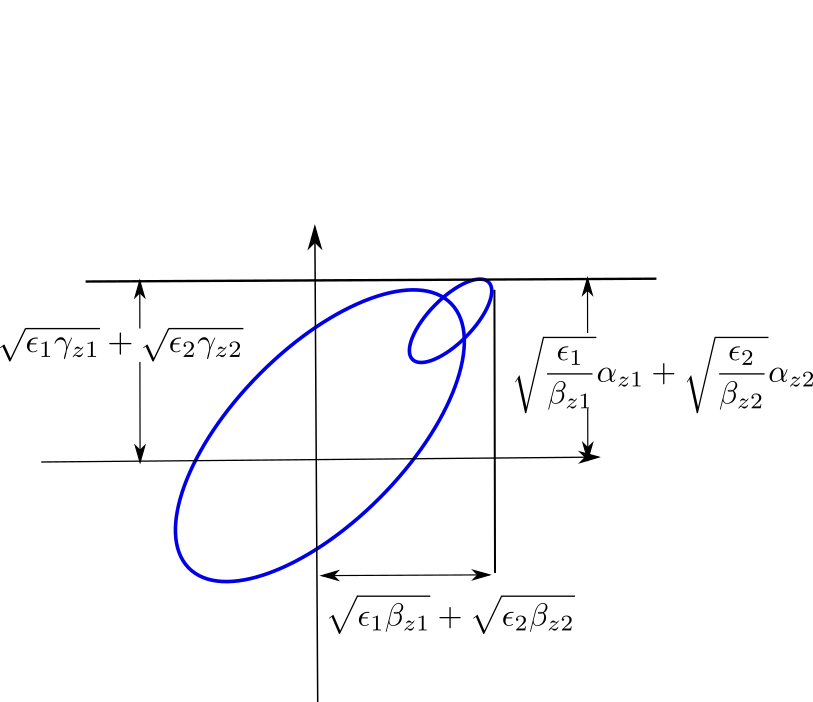
\includegraphics[width=1.0\linewidth]{ripken_phase_space_ellipse.png}
	\caption{Projection of lattice function in the $z-z'$ plane.\label{opt:fig:2}}
\end{figure}

Using Eqns.~\ref{opt:eqn:3:3}, \ref{opt:eqn:4:1}, \ref{opt:eqn:4:2} and $\cos(x+y)=\cos x\cos y-\sin x\sin y$, the coordinates $z(s)$ can be expressed by:
\begin{align}
z_{2j-1}(s)&=\sum_{k=1}^3 \sqrt{2I_k
\beta_{k,j}(s)}\cos{(\phi_{k,j}(s)+\phi_{k,0})}\\
z_{2j}(s)&=\sum_{k=1}^3 \sqrt{2I_k
\gamma_{k,j}(s)}\cos{(\bar\phi_{k,j}(s)+\phi_{k,0})}, \ j=1,\ldots,3
\end{align}
Conversely the lattice functions can also be expressed by $a_k$ and $b_k$ with
\begin{align}
\beta_{k,j}(s)&=a_{k,2j-1}(s)^2 +b_{k,2j-1}(s)^2 \\
\alpha_{k,j}(s)&=a_{k,2j-1}(s)a_{k,2j}(s) -b_{k,2j-1}(s)b_{k,2j}(s) \\
\gamma_{k,j}(s)&=a_{k,2j}(s)^2 +b_{k,2j}(s)^2,
\end{align}
The well known relations between the lattice functions
\begin{align}
\sum_{j=1}^3\beta_{k,j}\phi_{k,j}'&=1 \\
\gamma_{k,j}&=\frac{\beta_{k,j}^2\phi_{k,j}'^2+\alpha_{k,j}^2}{\beta_{k,j}}, \text{ with  }\\
\alpha_{k,j}&:=-\frac{1}{2}\beta_{k,j}'
\end{align}
can then be derived with the help of the normalization condition (Eqn.~\ref{opt:eqn:2:3})
\begin{align}
a_k^TSb_k=1
\end{align}
by the following steps:
\begin{enumerate}
\item As $x'=\frac{dx}{ds},\ y'=\frac{dy}{ds}$ and $\delta=\frac{d\sigma}{ds}$ the following relations hold also for $a_k$ and $b_k$:
\begin{align}
a_{k,2j}=a_{k,2j-1}'&=\frac{d}{ds}(a_{k,2j-1}), \\
b_{k,2j}=b_{k,2j-1}'&=\frac{d}{ds}(b_{k,2j-1}),\ k,j=1,\ldots,3 
\end{align}
\item The normalization condition Eqn.~\ref{opt:eqn:2:3} can then be written as
\begin{align}
a_k^TSb_k&=\sum_{j=1}^3\sqrt{\beta_{k,j}}\cos{\phi_{k,j}}\left(\sqrt{\beta_{k,j}}\sin{\phi_{k,j}}\right)'\nonumber\\
& \qquad -\left(\sqrt{\beta_{k,j}}\cos{\phi_{k,j}}\right)'\sqrt{\beta_{k,j}}\sin{\phi_{k,j}}\nonumber\\
&=\sum_{j=1}^3\beta_{k,j}\phi_{k,j}'\nonumber\\
&=1 \label{opt:eqn:4:3}
\end{align}
Note that Eqn.~\ref{opt:eqn:4:3} yields the the following relation between the phase advance $\phi$ and $\beta$ in 2D:
\begin{align}
\phi(s)=\phi(0)+\int_{s_0}^s\frac{1}{\beta(\bar s)}d\bar s
\end{align}
\item Using the abbreviation $\alpha_{k,j}:=-\frac{1}{2}\beta_{k,j}$, one finds for each mode $k$ and plane $j$
\begin{align}
\sqrt{\gamma_{k,j}}\cos{\phi_{k,j}}&=a_{k,2j}=a_{k,2j-1}'=(\sqrt{\beta_{k,j}}\cos{\phi_{k,j}})' &\quad (1)\nonumber\\
\sqrt{\gamma_{k,j}}\sin{\phi_{k,j}}&=b_{k,2j}=b_{k,2j-1}'=(\sqrt{\beta_{k,j}}\sin{\phi_{k,j}})' &\quad (2)\nonumber\\
\overset{(1)^2+(2)^2}{\Rightarrow} \gamma_{k,j}&=\frac{\beta_{k,j}^2\phi_{k,j}'^2+\alpha_{k,j}^2}{\beta_{k,j}}, \quad k,j=1,\ldots,3 &
\end{align}
which simplifies in the 2D case to:
\begin{align}
\gamma\overset{\rm Eqn.~\ref{opt:eqn:4:3}}{=}\frac{1+\alpha^2}{\beta}
\end{align}
\end{enumerate}


%\section{Beam Optics Calculations}
%
%The optical properties of a lattice are conveniently described by a set of
%lattice functions. For a general four dimensional case, including coupling,
%two distinct oscillation modes $I$ and $II$ gives rise to two sets of lattice
%functions. For mode $I$ in the horizontal plane the lattice functions are
%defined
%as \cite{beamoptics}
%\begin{itemize}
%    \item $\sqrt{\beta_{xI}(s)}$ is the envelope function.
%    \item $\cos\Phi_{xI}(s)$ and $\sin\Phi_{xI}(s)$ are the phase functions.
%    \item $\sqrt{\gamma_{xI}(s)}$ is the angular envelope function.
%    \item $\cos\tilde{\Phi}_{xI}(s)$ and $\sin\tilde{\Phi}_{xI}(s)$  are the
%  angular phase functions.
%\end{itemize}
%The lattice functions for mode $II$ are defined similarly, as well as for mode
%$I$ and $II$ in the vertical plane.

%A point in the four dimensional phase space $(x,x',y,y')$ can be described by
%four independent vectors $\vec{z}_i$ with coordinates $(x_i,x_i',y_i,y_i')$
%for $i=1,\ldots,4$.  Using the lattice functions these coordinates are
%expressed as
%\begin{align}
%    x_1 &= \sqrt{\beta_{xI}(s)}\cos\Phi_{xI}(s) & 
%    x_2 &= \sqrt{\beta_{xI}(s)}\sin\Phi_{xI}(s) \\
%    x'_1 &= \sqrt{\gamma_{xI}(s)}\cos\tilde{\Phi}_{xI}(s) & 
%    x'_2 &= \sqrt{\gamma_{xI}(s)}\sin\tilde{\Phi}_{xI}(s) \\
%    x_3 &= \sqrt{\beta_{xII}(s)}\cos\Phi_{xII}(s) & 
%    x_4 &= \sqrt{\beta_{xII}(s)}\sin\Phi_{xII}(s) \\
%    x'_3 &= \sqrt{\gamma_{xII}(s)}\cos\tilde{\Phi}_{xII}(s) & 
%    x'_4 &= \sqrt{\gamma_{xII}(s)}\sin\tilde{\Phi}_{xII}(s),
%\end{align}
%and similarly for the $y$- and $y'$-coordinates, using the lattice functions for the vertical plane.
%The trajectory in the four dimensional phase space can then be described as
%\begin{equation}
%    \vec{z} = \left(
%        \begin{array}{l}
%            \sqrt{\epsilon_I}\sqrt{\beta_{xI}}\cos(\Phi_{xI}+\phi_I) +
%            \sqrt{\epsilon_{II}}\sqrt{\beta_{xII}}\cos(\Phi_{xII}+\phi_{II}) \\
%            \sqrt{\epsilon_I}\sqrt{\gamma_{xI}}\cos(\tilde{\Phi}_{xI}+\phi_I) +
%            \sqrt{\epsilon_{II}}\sqrt{\gamma_{xII}}\cos(\tilde{\Phi}_{xII}+\phi_{II}) \\ 
%            \sqrt{\epsilon_I}\sqrt{\beta_{yI}}\cos(\Phi_{yI}+\phi_I) +
%            \sqrt{\epsilon_{II}}\sqrt{\beta_{yII}}\cos(\Phi_{yII}+\phi_{II}) \\
%            \sqrt{\epsilon_I}\sqrt{\gamma_{yI}}\cos(\tilde{\Phi}_{yI}+\phi_I) +
%            \sqrt{\epsilon_{II}}\sqrt{\gamma_{yII}}\cos(\tilde{\Phi}_{yII}+\phi_{II}) 
%        \end{array}
%    \right),
%\end{equation}
%where $\phi_I$ and $\phi_{II}$ are initial phases for the $I$ and $II$ mode,
%respectively. $\sqrt{\epsilon_{I}}$ and $\sqrt{\epsilon_{II}}$ are the
%amplitudes of mode $I$ and $II$, respectively.

%To calculate the lattice functions from the one-turn transfer map $M$ the 
%following procedure can be followed
%\begin{itemize}
%    \item Calculate the eigenvectors $\vec{v}_I$ and $\vec{v}_{II}$ and 
%    eigenvalues of $M$ at $s_0$.
%    \item Form the generating vectors
%        \begin{align*}
%            \vec{z}_{1,3} &= \frac{1}{\sqrt{2}} (\vec{v}_{I,II}
%                                +\vec{v}^*_{I,II}) \\
%            \vec{z}_{2,4} &= -\frac{i}{\sqrt{2}} (\vec{v}_{I,II}
%                                -\vec{v}^*_{I,II}) 
%        \end{align*}
%    \item Normalize the generating vectors according to 
%    $(\vec{z}_{1,3})^T S \vec{z}_{2,4}=1$
%    \item Calculate the initial lattice functions at $s_0$ by
%        \begin{equation*}
%            \left(
%                \begin{array}{cccc}
%                    \beta_{xI}=x_1^2+x_2^2 & \gamma_{xI}={x'}_1^2+{x'}_2^2 &
%                    \alpha_{xI}=-(x_1{x'}_1+x_2{x'}_2) & \Phi_{xI}=\arctan(x_2/x_1) \\
%                    \beta_{xII}=x_3^2+x_4^2 & \gamma_{xII}={x'}_3^2+{x'}_4^2 &
%                    \alpha_{xII}=-(x_3{x'}_3+x_4{x'}_4) & \Phi_{xII}=\arctan(x_4/x_3) \\ 
%                    \beta_{yI}=y_3^2+y_4^2 & \gamma_{yI}={y'}_3^2+{y'}_4^2 &
%                    \alpha_{yI}=-(y_3{y'}_3+y_4{y'}_4) & \Phi_{yI}=\arctan(y_4/y_3) \\
%                    \beta_{yII}=y_1^1+y_2^2 & \gamma_{yII}={y'}_1^2+{y'}_2^2 &
%                    \alpha_{yII}=-(y_1{y'}_1+y_2{y'}_2) & \Phi_{yII}=\arctan(y_2/y_1) 
%                \end{array}
%            \right)
%        \end{equation*}
%        where   $a_i=\frac{\partial{a}}{\partial{z_i}}$, that is, $x_1=\frac{\partial{x}}{\partial{x}},~x_2=\frac{\partial{x}}{\partial{x'}},~x_3=\frac{\partial{x}}{\partial{y}},...$ and so on.
%\end{itemize}

%\section{Optics Reference}
%A useful reference table describing the formulas that define the variables and the notation conventions to reference them can be found in the Table \ref{tab:opticsReference}.

%\begin{table}
%	\centering
%	\begin{tabular}{|l|l|l|}
%     \hline   	
%     \textbf{Symbol}& \textbf{Description} & \textbf{Formula} \\        \hline
%		N&Number of particles&\\
%		$z$&Particle characteristics&$z=\{x,x',y, y',\sigma,\delta\}$\\
%		$x,y$& x and y coordinates&\\
%		$p_x,p_y$& x and y momenta&\\
%		$\sigma$&Path length&$\sigma=s-v_0 \times t$\\
%		$\delta$&Relative momentum deviation&$\delta=\frac{\Delta P}{p_0}$\\
%               $M$&One-turn tracking Matrix&$M_{ij}=\frac{\partial z_i}{\partial z_j}$\\
%              $z_0$&Closed Orbit parameters&$z_0=\{x_0, {x_0}',y_0,{y_0}', \sigma_0, \delta_0\}$\\
%	$\tilde{z}$&Particle characteristics respect to the closed orbit&$\tilde{z}=\{\tilde{x},\tilde{x}',\tilde{y}, \tilde{y}',\tilde{\sigma},\tilde{\delta}\}$ where $\tilde{z_i}=z_i - z_0$ \\
%$\widetilde{x'},\widetilde{y'}$&Canonical momentums $\widetilde{x'},\widetilde{y'}$&$\{\widetilde{x'},\widetilde{y'}\}=\{x',y'\}*((1+\delta)+\delta_0)$\\
%		$Q_x$, $Q_y$&Horizontal and vertical tunes&\\
%		$Q'_x$, $Q'_y$&Horizontal and vertical chromaticities&\\
%		$\psi,\overline{\psi}$&Phase advance, Mean phase advance&\\
%	$\epsilon_x$& Horizontal emmitance&$\epsilon_x=c^2+\frac{\beta_{xI}*\widetilde{x'}+\alpha_{xI}*\tilde{x}}{\beta_{xI}}$\\
%    $\epsilon_y$& Vertical emmitance& $\epsilon_y=c^2+\frac{\beta_{yI}*\widetilde{y'}+\alpha_{yI}*\tilde{y}}{\beta_{yI}}$\\
%	$\overline{\epsilon}$& Averaged emmitance&\\
%	$\epsilon_I, \epsilon_{II}$&Mode I and Mode II emittances&$\epsilon_I=\epsilon_{vx}$, $\epsilon_{II}=\epsilon_{vy}$\\
%	$\epsilon_{vx}$&Linear decoupled horizontal emmitance&$\epsilon_{vx}=\left(\tilde{x}\sum^6_{i=0}M_{i,1}\right)^2+\left({x'}\sum^6_{i=0}M_{i,2}\right)^2$\\
%	$\epsilon_{vy},$&Linear decoupled vertical emmitance&$\epsilon_{vy}=\left(\tilde{y}\sum^6_{i=0}M_{i,3}\right)^2+\left(\widetilde{y'}\sum^6_{i=0}M_{i,4}\right)^2$\\
%	$\epsilon_{vt}$& Emmitance sum...&$\epsilon_{vt}=\epsilon_x+\epsilon_y$\\
%	$\beta_{xI}$&Primary horizontal $\beta $\-function&$\beta_{xI}={M_{1,1}}^2+{M_{1,2}}^2$\\
%    $\beta_{xII}$&Secondary horizontal $\beta $\-function&$\beta_{xII}={M_{1,3}}^2+{M_{1,4}}^2$\\
%	$\beta_{yI}$&Primary vertical $\beta $\-function&$\beta_{yI}={M_{3,3}}^2+{M_{3,4}}^2$\\
%    $\beta_{yII}$&Secondary vertical $\beta $\-function&$\beta_{yII}={M_{3,1}}^2+{M_{3,2}}^2$\\		
%		\hline
%\end{tabular}
%\caption{\label{tab:opticsReference}Optics Reference}
%\end{table}


%\section{Code naming conventions}

%\section{Notes on tracking programs}

%A particle tracking program for accelerators like Sixtrack is based on the
%concepts of beamline elements representing real devices (dipoles, quadrupole,
%cavities) and symplectic integrators using predefined maps (i.e.  solution of
%equations of motion).

%A map is a transformation of particle coordinates formulated is such a way
%that coordinates can be either floating point numbers or truncated
%polynomials. A map may reflect the effects of a field on a particle or a
%change of the reference frame or other even non physical transformations.

%An integrator solves the equations of motion of a particle under the influence
%of a specific force often generate by electromagnetic fields using some
%approximations. It is often coded as an explicit map or sequence of them.

%A particle trajectory in beam line element can equally well computed using
%different type of integrators depending on the initial coordinates and the
%application.

%For relativistic particles an integrator can be qualified in terms of:
%\begin{itemize}
%\item the longitudinal coordinate definition:
%  $(\Delta t,p_t)$,
%  $(\sigma,p_\sigma)$,
%  $(\Delta s, \delta)$.
%\item the approximation of the Hamiltonian: exact or expanded.
%\item the type of Hamiltonian splitting:
%\begin{itemize}
%  \item kick-drift,
%  \item matrix-kick: keep the linear motion of the original Hamiltonian exact,
%  \item no splitting: solving the motion exactly.
%\end{itemize}
%\item the order of the approximation in $s$.
%\item the integrations step inside an element.
%\end{itemize}

%Tracking codes can be used:
%\begin{itemize}
%  \item for tracking studies: compute the evolution of one or more particle
%    trajectories along beam-line elements for one or more turns and perform
%    post processing analysis (particle loss, frequency maps, invariant
%    reconstruction,...)
%  \item optics studies: compute the sensitivity of the particle trajectories
%    with respect to the initial conditions around a reference trajectories. It
%    can be implemented using TPSA algebraic operations  as substitute of
%    floating point ones or by explicit equations. Finite differences on real
%trajectories may be used as well at the cost of loosing precision on
%simplistic invariants.

%\end{itemize}

%In Sixtrack the build up of an integrator is left to the user when defining
%the lattice. An exact correspondence between beam line element is not necessarily needed. Sixtrack uses only one particular choice for the longitudinal Sixtrack uses only one particular choice for the longitudinal
%coordinates. It can be used for periodic structures only around one closed
%orbit. Sixtrack has the tools to compute linear and non-linear optics using
%matrix manipulation and TPSA, however it is not meant to be used as an
%interactive design tool like MAD-X.


\section{Table of symbols}

\begin{description}
\item $\vec R$: moving reference frame origin
\item $s$: path length of the reference frame origin trajectory
\item $\hat X, \hat Y,\hat Z$: global reference frame bases
\item $X, Y, Z$: reference frame origin coordinates $\vec R(s)=X(s) \hat X+Y(s) \hat Y+ Z(s) \hat Z$
\item $\vec Q$: particle position
\item $\hat x, \hat y, \hat s$: moving reference frame bases
\item $x, y$: transverse particle coordinates $\vec Q(s)= \vec R(s) + x(s) \,\hat x(s) + y(s)\, \hat y(s)$
\item $t(s)$: time at which the particle is located in the plane $\hat x(s), \hat y(s)$
\item $v, P, E, m, q$: particle velocity momenta, energy, rest mass, charge
\item $v_0, P_0, E_0, m_0, q_0$: reference momentum, energy, rest mass,
\item $\beta_0, \gamma_0$: reference relativistic factors
\item $\Delta t=s/\beta_0 - c t$: Mad time deviation, canonical conjugate of $p_t$
\item $\sigma=s - \beta_0 c t$: Sixtrack time deviation, canonical conjugate of $p_\sigma$
\item $\Delta s=s - \beta c t  $  path length deviation, canonical conjugate of $\delta$
\item $z=\beta(s/\beta_0 - c t) $  John time deviation, canonical conjugate of $\delta$
\item $\rho=1/h$ Radius of curvature for a moving reference frame in a circular trajectory. 
\item $P_x, P_y,  P_s$: canonical momenta coordinates in a straight or curved reference frame. Note that for a circular trajectory: $v_s= (1 +h x) \dot s$, $P_x=m \gamma \dot x + q A_x$, $P_y=m \gamma \dot y q A_y$ and 
$P_s=m \gamma \dot s (1 + h x)^2 + q (1 + h x) A_s$.
\item $p_x=P_x/P_0, p_y=P_x/P_0, p_s=P_s/P_0$ normalized momenta coordinates
\item $x'=P_x/P_s,y'=P_x/P_s$ transverse divergence coordinates
\item $x_p=P_x/P,y_p=P_y/P$ approximated divergence coordinates
\item $\delta=(P-P_0)/P_0$: normalized momentum deviation
\item $p_t=(E-E_0)/P_0c$: normalized energy deviation
\item $p_\sigma=(E-E_0)/\beta_0 P_0c$: SixTrack energy deviation canonical conjugate of $\sigma$
\item $H$ Hamiltonian function
\item $E_x, E_y, E_s$ Electric fields in a straight or curved reference frame
\item $B_x, B_y, B_s$ Magnetic fluxes in a straight or curved reference frame
\item $A_x, A_y, A_s$ Magnetic fluxes in a straight or curved reference frame
\end{description}


\bibliographystyle{unsrt}
\bibliography{bibliography}

\end{document}
